\documentclass[12pt,a4paper,oneside]{report}

% =========================================================
% INSTRUCTIONS FOR OVERLEAF COMPILATION:
% 1. Go to Overleaf -> Menu (top-left) -> Settings
% 2. Set 'Compiler' to 'XeLaTeX' (for native Unicode & Vietnamese fonts)
% =========================================================

% ---------------------------------------------------------
% Core Academic Packages & Engine Configuration
% ---------------------------------------------------------
\usepackage{iftex}
\ifPDFTeX
  \usepackage[utf8]{inputenc}
  \usepackage[T5,T1]{fontenc}
  \usepackage{lmodern}
\else
  % Compile with XeLaTeX on Overleaf
  \usepackage{fontspec}
  \defaultfontfeatures{Ligatures=TeX}
  \setmainfont{Noto Serif}
\fi

\usepackage[margin=1in]{geometry}
\usepackage{amsmath,amssymb,amsfonts}
\usepackage{booktabs}
\usepackage{array}
\usepackage{multirow}
\usepackage{graphicx}
\usepackage{xcolor}
\usepackage{subcaption}
\usepackage{cite}
\usepackage{listings}
\usepackage{microtype}
\usepackage{setspace}
\usepackage{titlesec}
\usepackage{enumitem}
\usepackage[ruled,vlined,linesnumbered]{algorithm2e}
\usepackage{tikz}
\usetikzlibrary{shapes.geometric, arrows.meta, positioning, calc}
\usepackage[hidelinks,breaklinks=true,pdfencoding=auto]{hyperref}

% Typography & Spacing
\onehalfspacing
\setlength{\parindent}{1.5em}
\setlength{\parskip}{0.5em}

% Custom Colors for Tables and Highlights
\definecolor{aetronblue}{RGB}{20, 55, 94}
\definecolor{aetroncyan}{RGB}{47, 138, 175}
\definecolor{codegreen}{RGB}{40, 140, 70}
\definecolor{codegray}{RGB}{120, 120, 120}

% Title Formatting
\titleformat{\chapter}[display]
  {\normalfont\bfseries\color{aetronblue}}
  {\filleft\fontsize{14}{14}\selectfont CHAPTER \thechapter}
  {1ex}
  {\titlerule\vspace{1ex}\LARGE}
  [\vspace{1ex}\titlerule]

\titlespacing*{\chapter}{0pt}{20pt}{25pt}

% ---------------------------------------------------------
% Document Metadata
% ---------------------------------------------------------
\title{\textbf{AETRON: A RESEARCH-DRIVEN MULTI-MODAL MOBILE FITNESS TRACKING PLATFORM WITH EMPIRICAL ALGORITHMIC BENCHMARKING}}
\author{Nguyễn Đức Bảo (Student ID: ITITIU22238)}
\date{November 2026}

\begin{document}

% ---------------------------------------------------------
% Front Matter
% ---------------------------------------------------------
\begin{titlepage}
    \centering
    \vspace*{0.5cm}

    {\fontsize{13}{15}\selectfont \textbf{VIETNAM NATIONAL UNIVERSITY -- HO CHI MINH CITY}}\\
    {\fontsize{13}{15}\selectfont \textbf{INTERNATIONAL UNIVERSITY}}\\
    {\fontsize{12}{14}\selectfont \textbf{SCHOOL OF COMPUTER SCIENCE AND ENGINEERING}}\\
    {\fontsize{11}{13}\selectfont \textbf{DEPARTMENT OF INFORMATION TECHNOLOGY}}\\[1.8cm]

    % University Logo / Crest (Gracefully handles absence of local image)
    \IfFileExists{figures/iu_logo.png}{%
        
\includegraphics[width=0.22\textwidth]{figures/iu_logo.png}\\[1.5cm]
    }{%
        \vspace{3.5cm}%
    }

    {\fontsize{16}{20}\selectfont \textbf{GRADUATION THESIS}}\\[0.8cm]

    {\fontsize{15}{19}\selectfont \textbf{AETRON: A RESEARCH-DRIVEN MULTI-MODAL MOBILE FITNESS TRACKING PLATFORM WITH EMPIRICAL ALGORITHMIC BENCHMARKING}}\\[2.0cm]

    \begin{minipage}{0.85\textwidth}
        \begin{tabular}{ll}
            \textbf{Author:} & Nguyễn Đức Bảo (ITITIU22238) \\
            \textbf{Program:} & Bachelor of Science in Information Technology \\
            \textbf{Department:} & School of Computer Science and Engineering \\
            \textbf{Academic Year:} & 2022 -- 2026 \\
        \end{tabular}
    \end{minipage}

    \vfill
    {\fontsize{11}{13}\selectfont Ho Chi Minh City, November 2026}
\end{titlepage}

\newpage
\pagenumbering{roman}

% ---------------------------------------------------------
% Abstract
% ---------------------------------------------------------
\chapter*{Abstract}
\addcontentsline{toc}{chapter}{Abstract}
Modern mobile fitness applications require robust, real-time sensory telemetry across heterogeneous indoor and outdoor physical environments. However, consumer smartphones face severe sensing constraints: satellite signal degradation and multipath errors in urban canyons, mobile operating system sandboxing that blocks ambient light and raw radio APIs on iOS, rapid state oscillation across indoor--outdoor boundaries, false step counts triggered by stationary device handling, and display jitter during live biomechanical cadence feedback. While commercial platforms (e.g., Strava, Nike Run Club) deliver polished user experiences, their core filtering and sensing pipelines remain proprietary black boxes.

This thesis presents \textbf{Aetron}, an open, research-grounded, multi-modal mobile fitness tracking platform built on Flutter and Dart for native Android and iOS devices. Aetron unifies real-time sensor fusion with rigorous offline scientific validation across six algorithmic subsystems grounded in peer-reviewed literature: (1)~an outdoor 4-state 2D kinematic Extended Kalman Filter (EKF) with Joseph-form covariance stabilization, Zero-Velocity Update (ZUPT), and Phase~1/2 kinematic preprocessing and Mahalanobis gating; (2)~a cross-platform Indoor--Outdoor Detection (IOD) architecture pairing an Android 4-channel 2D Depthwise Separable CNN (Model~C-Mobile) and an Adaptive Transition Engine with an \textbf{iOS-first light-free multi-sensor classifier} combining MagIO geomagnetic perturbation features, linear acceleration dynamics, CoreLocation accuracy/outage likelihoods, \texttt{CMAltimeter} barometric pressure deltas, and a causal 2-state Hidden Markov Model (HMM) alongside a probabilistic path-straightness \texttt{EnvironmentClassifier}; (3)~causal inertial step detectors (Oxford WPD for walking and Xu FFT-adaptive detection for running) hardened with Skog et al.'s Magnitude-Variance Generalized Likelihood Ratio Test (MV-GLRT) ZUPT, Brajdic \& Harle rhythmic bout gating, a 6-second sliding-window cadence engine, and Leave-One-Subject-Out (LOSO) Renaudin adaptive step-length estimation; (4)~offline display-only trajectory reconstruction comparing Linear Chord and Monotone PCHIP interpolation; (5)~T-DBSCAN spatial--temporal dwell clustering and Google Encoded Polyline compression; and (6)~2024 Adult Compendium speed-banded metabolic expenditure modeling with client--server parity.

All subsystems are audited against published public datasets with independent physical ground truth: TU~Wien Leica GS18 phase-RTK pedestrian walks, Oxford SnapperGPS~2 cycling tracks, Cambridge CIOD and HAR-PMD environmental traces ($>490{,}000$ epochs), STAGA mobility diaries ($122{,}808$ epochs), Clemson PedEval and Oxford OxWalk ($119{,}572$ video-annotated steps), Oxford WPD and Xu Group~3 accelerometry, and SLEDataset2 / Fukuchi RBDS stride-length cohorts. Rigorous holdout testing yields actionable and transparent findings: on TU~Wien RTK walks, isolating NIS scaling alone over a tuned EKF fails the predefined $10\%$ acceptance gate ($+0.21\%$ RMSE change, 95\% cluster bootstrap CI $[-0.0233, +0.0034]$\,m), whereas coupling Phase~1 preprocessing with Phase~2 Mahalanobis-gated 4-state AEKF resolves the legacy Fixed-Alpha stationary-freeze pathology ($8.753$\,m $\to 3.432$\,m RMSE; $1.34\%$ contiguous distance error), while SnapperGPS cycling under CEP50 without Doppler exposes a critical negative result ($138.226$\,m RMSE). On held-out Cambridge CIOD (Sessions~72--84, $N=201{,}731$), our iOS-compatible light-free \texttt{[MagIO+Acc+Daytime]} MLP achieves \textbf{77.07\% accuracy} and \textbf{74.97\% Macro-F1} ($75.65\%$ / $74.77\%$ with causal HMM and $69.48\%$ outdoor recall), outperforming the Android-only 4-channel baseline ($73.64\%$ / $69.59\%$) while restoring 100\% sensor coverage on iOS; meanwhile, event-level doorway transition F1 remains modest ($4.39\%$, $15/46$ physical transits), enforcing \texttt{isObservationalOnly: true} in production. Finally, MV-GLRT ZUPT eliminates 100\% of stationary hand-sway and $2.2$\,m/s$^2$ screen-tap false steps ($0$ false steps over $60$\,s) while preserving $4{,}225/4{,}107$ steps on Oxford WPD and $1{,}265/1{,}280$ on Xu Group~3, and the 6-second cadence window cuts display flutter by $50.0\%$ with $8.41$\,spm steady-state MAE.

\vspace{0.8cm}
\noindent\textbf{Keywords:} Mobile Fitness Tracking, Extended Kalman Filter (EKF), Indoor/Outdoor Detection (IOD), MagIO, Hidden Markov Model, Zero-Velocity Update (MV-GLRT), Biomechanical Cadence, Reproducible Benchmarking.

% ---------------------------------------------------------
% Table of Contents & Lists
% ---------------------------------------------------------
\tableofcontents
\listoffigures
\listoftables

\newpage
\pagenumbering{arabic}

% ---------------------------------------------------------
% Chapters Inclusion
% ---------------------------------------------------------
\chapter{Introduction}
\label{ch:introduction}

\section{Background}
Smartphone-based fitness tracking applications have become everyday tools for helping individuals monitor aerobic exercise, establish consistent training routines, and quantify energy expenditure. Modern consumer smartphones integrate all necessary telemetry hardware in a single pocketable device: multi-constellation Global Navigation Satellite System (GNSS) receivers, 3-axis MEMS accelerometers and gyroscopes, 3-axis magnetometers, barometric pressure sensors, and operating-system motion co-processors. Because workouts span both open-air environments (parks, urban streets, running tracks) and GPS-denied indoor spaces (gyms, treadmills, covered walkways), a reliable mobile fitness platform must adapt seamlessly between outdoor positioning and indoor inertial dead reckoning without requiring external chest straps or dedicated running watches.

While commercial platforms such as Strava, Nike Run Club, Samsung Health, and Google Fit demonstrate compelling user experiences, their core filtering pipelines, indoor/outdoor transition triggers, step gating heuristics, and calorie scaling factors remain proprietary. Conversely, existing student and open-source mobile fitness projects typically implement isolated fragments---rendering raw polylines directly on a map or polling an unguarded pedometer stream---without addressing urban GNSS drift, operating-system sensor restrictions, stationary false steps, crash-safe local storage, or multi-screen metric synchronization.

The application developed in this thesis is named \textbf{Aetron}. Implemented in Flutter~\cite{flutter2024framework} using a single Dart codebase targeting native Android and iOS devices, Aetron unifies live sensor fusion with offline-first persistence and cloud reconciliation. Location streams are ingested via \texttt{geolocator}~\cite{geolocator2024}, native step counters via \texttt{pedometer}~\cite{pedometer2024} alongside direct triaxial inertial pipelines, reactive state via Riverpod~\cite{riverpod2024state}, local telemetry persistence via Isar~\cite{isar2024database} and SQLite (\texttt{sqflite})~\cite{sqflite2024}, and synchronization plus server-side canonical finalization via Supabase~\cite{supabase2024backend}. Building upon an earlier deterministic pre-thesis baseline~\cite{aetron2026prethesis}, this graduation thesis advances Aetron from heuristic thresholds to peer-reviewed, mathematically grounded algorithms verified against both field trials and open public benchmark datasets.

\section{Problem Statement}
Implementing an accurate, cross-platform fitness tracker exclusively on commodity Android and iOS hardware remains technically demanding because every sensor modality exhibits failure modes across indoor and outdoor settings. GNSS signals degrade severely in urban canyons and fail inside buildings~\cite{merry2019gps,zandbergen2011gps}; hardware pedometers and software peak detectors accumulate false steps when users tap the screen or handle the phone while standing still; operating systems---most notably Apple iOS---strictly sandbox ambient light sensors, cellular radio metrics, and raw satellite carrier-to-noise density; and mobile background execution faces abrupt OS termination.

From a systems and algorithmic perspective, the core problem addressed by this thesis is:
\begin{quote}
\textit{Design, implement, and empirically validate a cross-platform mobile fitness tracking application that accurately captures indoor and outdoor workout sessions, performs robust environment classification across heterogeneous Android and iOS sensor constraints, computes consistent real-time and post-workout telemetry, guarantees crash-resilient offline-first persistence with verifiable cloud reconciliation, and maintains uniform metrics across all application modules.}
\end{quote}

Specifically, the system must resolve five coupled engineering and scientific challenges:
\begin{enumerate}
    \item \textbf{Outdoor GNSS Noise, Multipath Drift, and Estimator Validation:} Smartphone location fixes exhibit stationary wander, multipath jumps, and urban-canyon degradation. A naive fixed-alpha exponential smoother risks freezing real movement at $1$\,Hz, whereas complex adaptive Kalman filters must be empirically verified against independent surveyor-grade ground truth rather than assumed to improve accuracy unconditionally.
    \item \textbf{Cross-Platform Indoor/Outdoor Detection (IOD) under iOS Sandboxing:} Lighting-dependent deep IOD models fail with $0\%$ coverage on iOS because third-party iOS apps cannot query the ambient light sensor or raw GNSS $C/N_0$. Moreover, instantaneous predictions suffer rapid boundary oscillation and activity confounding (misclassifying indoor walking as outdoor locomotion), requiring both light-free multi-sensor modeling and strict safety isolation.
    \item \textbf{Stationary False-Step Rejection and Cadence Stability:} Naive peak-detection and unguarded pedometer streams increment phantom steps during screen interaction or idle sway. Simultaneously, live cadence estimation requires balancing accuracy, second-to-second visual flutter, and stop-decay latency, while static stride constants misestimate varying walking and running speeds.
    \item \textbf{Metric Authority and Physiological Consistency:} Elapsed duration, moving time, pace, distance, cadence, and estimated calories must remain coherent from live recording through post-workout summary, history calendar, analytics charts, detail views, and backend verification---using transparent peer-reviewed lookup standards rather than ad-hoc scaling multipliers.
    \item \textbf{Local-First Durability and Multi-Account Integrity:} Recorded sessions and raw sensor points must survive OS kills, app restarts, connectivity loss, and account switching without losing finalized records or leaking records across signed-in accounts.
\end{enumerate}

\section{Scope and Objectives}
Aetron targets individual users recording outdoor and indoor walking, running, cycling, and gym sessions solely with a smartphone. The application includes multi-modal Flutter/Dart client modules (Home, Activity/Recording, History/Calendar, Analytics, Profile, Goals, and Settings), offline-first Isar/SQLite storage, asynchronous Supabase synchronization, Deno post-processing workers, and a reproducible Python/Dart scientific benchmark suite.

To keep empirical claims honest, the project explicitly excludes: dedicated smartwatch or chest-strap heart-rate integration; clinical indirect calorimetry ($\dot{V}\text{O}_2$ testing)---caloric outputs are explicitly presented as population-average estimates; and production road-network map matching, where an OpenStreetMap/OSRM routing engine is not currently attached (so backend workers transparently report \texttt{routeMatchingAvailable() = false}).

The main objectives of this thesis extend the four pre-thesis goals (\textbf{O1}--\textbf{O4}) and establish formal scientific benchmarking (\textbf{O5}):
\begin{itemize}
    \item \textbf{O1 --- Adaptive Environment Classification and Safe Sensor Routing:} Pair a probabilistic \texttt{EnvironmentClassifier} (sigmoid GNSS likelihoods, Benhamou straightness, causal HMM, and iOS GPS-blackout detection) with cross-platform IOD classifiers (Android 4-channel Model~C-Mobile + Adaptive Transition Engine and iOS-first light-free MagIO + Accelerometer + CoreLocation + Barometer + HMM fusion), enforcing \texttt{isObservationalOnly = true} on experimental models so unverified flips never corrupt workout tracking.
    \item \textbf{O2 --- Research-Grounded Outdoor and Indoor Tracking Pipelines:} Upgrade outdoor filtering to a Joseph-stabilized 4-state kinematic EKF with ZUPT, Phase~1 preprocessing, Phase~2 Mahalanobis NIS gating, T-DBSCAN dwell suppression, and display-only PCHIP outage reconstruction; harden indoor pedometry using causal Oxford WPD and Xu Running detectors with Skog MV-GLRT stance rejection, Brajdic \& Harle \texttt{StepMotionGate}, a 6-second sliding cadence window, and LOSO-validated Renaudin stride estimation.
    \item \textbf{O3 --- Real-Time Session Experience and Caloric Parity:} Maintain live telemetry updates at $\le 1$\,s intervals across a refined Kinetic editorial UI with iOS Live Activities and direct iOS/Android OS notification settings deep-linking, paired with bit-exact 2024 Adult Compendium speed-banded caloric estimation across client and server.
    \item \textbf{O4 --- Crash-Resilient Persistence and Server Reconciliation:} Guarantee local-first Isar persistence with 5-second incremental checkpoints and account-scoped access checks before cloud synchronization, backed by idempotent Supabase PostgreSQL guards and Deno verification workers.
    \item \textbf{O5 --- Empirical Benchmarking, Negative-Result Disclosure, and Automated Verification:} Retain field comparisons against commercial apps alongside rigorous holdout evaluations on open ground-truth datasets (TU~Wien RTK, SnapperGPS~2, Cambridge CIOD, HAR-PMD, STAGA, PedEval, OxWalk, Oxford WPD, Xu Group~3, SLEDataset2, and Fukuchi RBDS), disclose negative results transparently, and maintain green CI (\texttt{0} analyzer issues and full regression test pass).
\end{itemize}

\section{Assumptions and Constraints}
\begin{enumerate}
    \item \textbf{Permissions and Sensor Availability:} Full dual-mode operation assumes the user grants foreground/background location, activity recognition (Android), motion \& fitness (iOS), and optional notification permissions. Notification preferences in settings are synchronized bidirectionally with OS-level authorization state.
    \item \textbf{Platform Sandboxing Constraints:} Apple iOS restricts third-party access to raw ambient illuminance, cellular signal parameters (RSRP/RSRQ), and raw GNSS carrier-phase/$C/N_0$ measurements; therefore, iOS classifiers rely strictly on public \texttt{CMMotionManager}, \texttt{CoreLocation}, and \texttt{CMAltimeter} streams.
    \item \textbf{Biomechanical and Metabolic Boundaries:} Without wearable heart-rate or metabolic-cart equipment, indoor distance from accelerometer/pedometer streams and kilocalorie estimates from 2024 Compendium MET tables represent statistical population approximations rather than individualized clinical measurements.
    \item \textbf{Hardware and Backend Resource Constraints:} Consumer smartphone GNSS accuracy remains constrained by multipath reflections and receiver antennas; backend deployments operate within Supabase database/worker limits without third-party commercial map-matching APIs.
\end{enumerate}

\section{Proposed Solution}
Aetron resolves these challenges through an offline-first, layered architecture combining real-time pure-Dart sensor fusion with transparent backend auditing and rigorous offline verification. At session start, \texttt{WorkoutSessionNotifier} initializes parallel location and motion pipelines alongside the passive \texttt{IodController} observational monitor. Depending on activity modality and real-time classification, verified GNSS updates flow through Phase~1 preprocessing and the 4-state kinematic EKF (or snapshot ZUPT/DBSCAN dwell guards), while indoor or GPS-denied intervals rely on MV-GLRT and \texttt{StepMotionGate}-hardened pedometry with Renaudin adaptive step length.

Every 5 seconds after meaningful progress and at workout completion, states are committed transactionally to Isar before entering the resilient synchronization queue to Supabase and \texttt{deterministic-finalize-worker}. Figure~\ref{fig:proposed_pipeline} illustrates the high-level indoor and outdoor workout data processing pipeline.

\begin{figure}[htbp]
\centering
\noindent\resizebox{0.94\textwidth}{!}{%
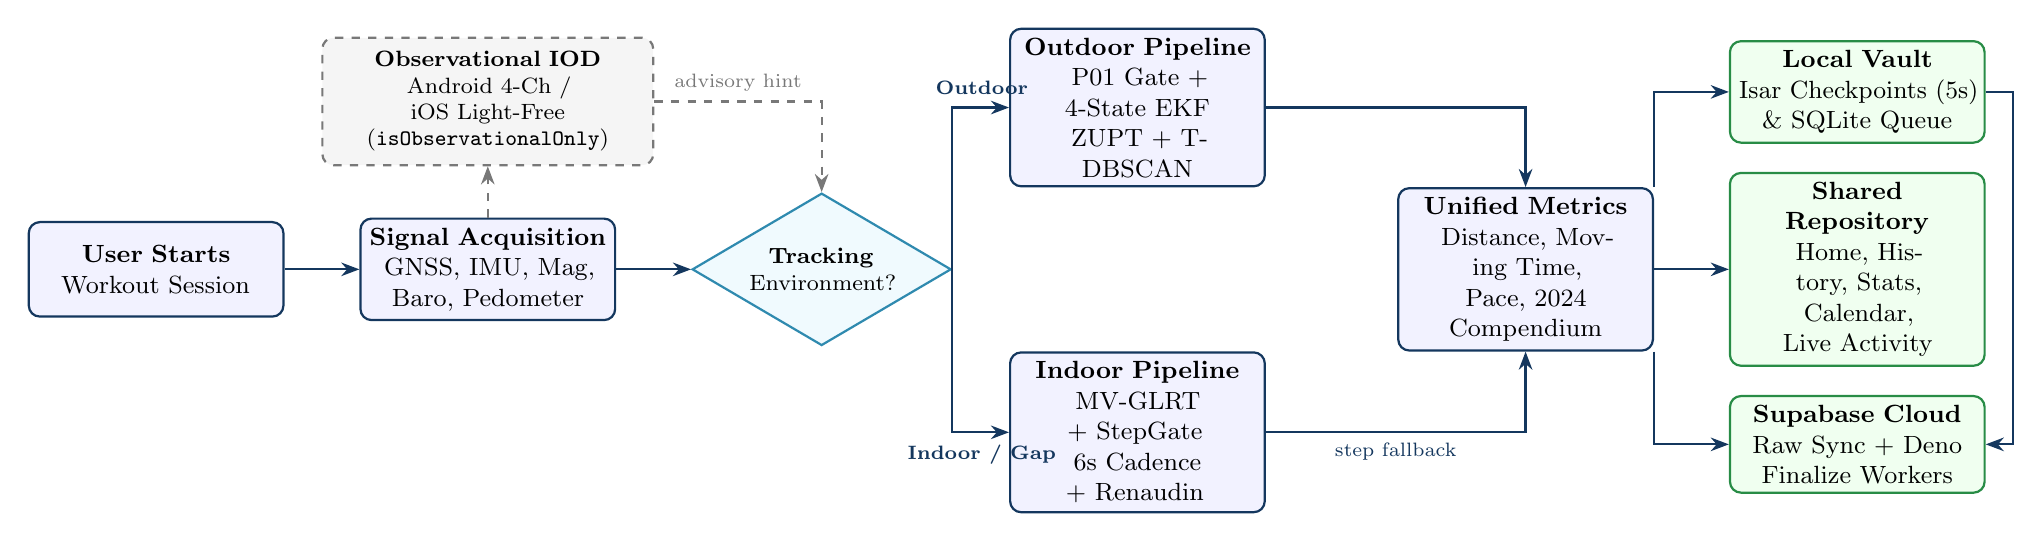
\begin{tikzpicture}[
    node distance=0.85cm and 0.95cm,
    box/.style={rectangle, rounded corners=4pt, draw=aetronblue, fill=blue!5, thick, text width=3.0cm, minimum height=1.2cm, align=center, font=\small},
    decision/.style={diamond, aspect=1.7, draw=aetroncyan, fill=cyan!6, thick, text width=2.2cm, align=center, font=\footnotesize, inner sep=1pt},
    obs/.style={rectangle, rounded corners=4pt, dashed, draw=codegray, fill=gray!8, thick, text width=3.85cm, align=center, font=\footnotesize, inner sep=5pt},
    storage/.style={rectangle, rounded corners=4pt, draw=codegreen, fill=green!6, thick, text width=3.0cm, minimum height=1.0cm, align=center, font=\small},
    arrow/.style={-{Stealth[length=2.3mm]}, thick, color=aetronblue}
]
    \node[box] (start) {\textbf{User Starts}\\Workout Session};
    \node[box, right=of start] (acq) {\textbf{Signal Acquisition}\\GNSS, IMU, Mag,\\Baro, Pedometer};
    \node[decision, right=of acq] (env) {\textbf{Tracking}\\Environment?};

    \node[box, above right=0.55cm and 1.55cm of env] (out) {\textbf{Outdoor Pipeline}\\P01 Gate + 4-State EKF\\ZUPT + T-DBSCAN};
    \node[box, below right=0.55cm and 1.55cm of env] (in) {\textbf{Indoor Pipeline}\\MV-GLRT + StepGate\\6s Cadence + Renaudin};

    \node[obs, above=0.65cm of acq] (iod) {\textbf{Observational IOD}\\Android 4-Ch / iOS Light-Free\\(\texttt{isObservationalOnly})};

    \node[box, right=5.65cm of env] (met) {\textbf{Unified Metrics}\\Distance, Moving Time,\\Pace, 2024 Compendium};

    \node[storage, above right=0.55cm and 0.95cm of met] (isar) {\textbf{Local Vault}\\Isar Checkpoints (5s)\\\& SQLite Queue};
    \node[storage, right=0.95cm of met] (ui) {\textbf{Shared Repository}\\Home, History, Stats,\\Calendar, Live Activity};
    \node[storage, below right=0.55cm and 0.95cm of met] (cloud) {\textbf{Supabase Cloud}\\Raw Sync + Deno\\Finalize Workers};

    \draw[arrow] (start) -- (acq);
    \draw[arrow] (acq) -- (env);
    \draw[arrow, dashed, color=codegray] (acq) -- (iod);
    \draw[arrow, dashed, color=codegray] (iod) -| node[pos=0.25, above, font=\scriptsize, color=codegray]{advisory hint} (env.north);

    \draw[arrow] (env.east) |- node[pos=0.76, above=1pt, font=\scriptsize\bfseries]{Outdoor} (out.west);
    \draw[arrow] (env.east) |- node[pos=0.76, below=1pt, font=\scriptsize\bfseries]{Indoor / Gap} (in.west);

    \draw[arrow] (out.east) -| (met.north);
    \draw[arrow] (in.east) -| node[pos=0.25, below, font=\scriptsize]{step fallback} (met.south);

    \draw[arrow] (met) -- (ui);
    \draw[arrow] (met.north east) |- (isar.west);
    \draw[arrow] (isar.east) -- ++(0.35,0) |- (cloud.east);
    \draw[arrow] (met.south east) |- (cloud.west);
\end{tikzpicture}%
}
\caption{End-to-end workout tracking data processing pipeline across outdoor GNSS filtering, indoor inertial pedometry, observational IOD monitoring, local persistence, and cloud reconciliation.}
\label{fig:proposed_pipeline}
\end{figure}

\section{Structure of the Thesis}
This thesis is organized into five chapters:
\begin{itemize}
    \item \textbf{Chapter~1 (Introduction):} Presents the project background, problem statement across indoor and outdoor mobile sensing, scope and objectives (\textbf{O1}--\textbf{O5}), assumptions and constraints, and the proposed end-to-end pipeline.
    \item \textbf{Chapter~2 (Literature Review):} Reviews the mathematical and empirical foundations of outdoor GNSS kinematics, EKF/AEKF and trajectory mining, cross-platform IOD under iOS/Android constraints, MV-GLRT stationary rejection, adaptive stride estimation, 2024 Adult Compendium calorimetry, commercial application baselines, and open research gaps.
    \item \textbf{Chapter~3 (System Design and Implementation):} Details Aetron's Clean Architecture, local Isar/SQLite and Supabase PostgreSQL schemas, probabilistic and multi-sensor IOD engines, 4-state EKF and P01/P02/P03/T-DBSCAN tracking pipelines, MV-GLRT indoor step/cadence system, synchronization and worker reconciliation, cross-screen data consistency, and UX/OS integration.
    \item \textbf{Chapter~4 (Experiment Results and Evaluation):} Reports both live smartphone comparisons (six commercial apps and $800$\,m MAPE) and comprehensive holdout benchmarks on public ground-truth datasets, including disciplined negative-result disclosures, execution profiling, automated regression test counts, and evaluation against objectives \textbf{O1}--\textbf{O5}.
    \item \textbf{Chapter~5 (Conclusion and Future Work):} Summarizes key contributions, critically discloses limitations and threats to validity, and outlines concrete future research steps.
\end{itemize}

\chapter{Literature Review}
\label{ch:literature_review}

\section{Overview}
This chapter reviews the technical foundations underpinning Aetron's design as a smartphone-only mobile fitness application for indoor and outdoor activities. Rather than relying on dedicated chest straps or proprietary smartwatch firmware, Aetron derives all motion, location, and metabolic telemetry from consumer smartphone GNSS receivers, micro-electro-mechanical (MEMS) inertial sensors, magnetometers, barometers, and platform OS APIs. The review connects classic mobile systems literature---used to frame our initial pre-thesis baseline---with peer-reviewed research in geodetic Kalman estimation, cross-platform Indoor/Outdoor Detection (IOD), zero-velocity gait gating, adaptive stride biomechanics, and exercise physiology.

\section{Mobile Fitness Tracking Applications}
Smartphone fitness applications transform raw heterogeneous hardware sensor streams into actionable workout metrics---distance, pace, cadence, steps, elevation, routes, and estimated calorie burn---without requiring external sports accessories. Building an academically transparent mobile tracker presents a systems integration challenge as much as an algorithmic one: sensor noise filtering, environment switching, crash-safe storage, server auditability, and reactive multi-screen presentation must operate coherently on battery-constrained phones.

\section{Outdoor Activity Tracking Using GPS/GNSS}
\label{sec:gnss_kinematics}

\subsection{GPS/GNSS as the Primary Outdoor Source}
Outdoor tracking relies on Global Navigation Satellite Systems (GPS, GLONASS, Galileo, BeiDou) exposed in Flutter via \texttt{geolocator}~\cite{geolocator2024} over Android \texttt{FusedLocationProvider} and iOS \texttt{CoreLocation}. Each position fix supplies WGS84 geodetic coordinates $(\phi_k, \lambda_k)$, altitude $h_k$, Doppler or derived ground speed $v_k$, bearing $\theta_k$, and a horizontal accuracy radius estimate $\sigma_{\text{acc}, k}$ (typically a $1\sigma$ / $68\%$ radial confidence estimate on native Android/iOS, in contrast to $50\%$ CEP50 reported by low-cost snapshot loggers~\cite{beuchert2023snappergps}). Native accuracy estimates serve both as noise variance priors inside Kalman filtering and as primary cues for outdoor/indoor classification.

\subsection{GPS Accuracy Limitations and Urban Multipath}
Commodity smartphone GNSS antennas suffer from low gain, linear polarization, ionospheric/tropospheric propagation delays, and severe non-line-of-sight (NLOS) multipath reflections near tall buildings~\cite{merry2019gps,zandbergen2011gps,yun2022gnss}. Merry and Bettinger~\cite{merry2019gps} observed consumer smartphone horizontal errors of $3$--$10$\,m under open sky escalating to $30$--$50$\,m in urban canyons, while Zandbergen and Barbeau~\cite{zandbergen2011gps} documented median A-GPS errors of $5$--$8.5$\,m outdoors degrading indoors to tens of meters. Poor satellite geometry quantified by Horizontal Dilution of Precision ($\sigma_{\text{pos}} = \text{HDOP} \cdot \sigma_{\text{pr}}$) further induces four classic fitness telemetry failures: stationary phantom drift during traffic-light pauses, transient multipath spikes, temporary blackouts under tree cover or bridges, and physically impossible speed bursts.

\subsection{Distance Calculation: Haversine, Vincenty, and Validation Benchmarks}
Consecutive validated WGS84 coordinates $p_k = (\phi_k, \lambda_k)$ and $p_{k+1} = (\phi_{k+1}, \lambda_{k+1})$ (in radians) are integrated along a trajectory via the great-circle Haversine formula~\cite{sinnott1984virtues}:
\begin{align}
    a &= \sin^2\!\left(\frac{\phi_{k+1}-\phi_k}{2}\right) + \cos(\phi_k)\cos(\phi_{k+1})\sin^2\!\left(\frac{\lambda_{k+1}-\lambda_k}{2}\right), \\
    c &= 2 \arctan2\!\left(\sqrt{a}, \sqrt{1-a}\right), \qquad d_{\text{seg}} = R_{\text{earth}} \cdot c,
    \label{eq:haversine}
\end{align}
with mean Earth radius $R_{\text{earth}} \approx 6{,}371{,}000$\,m and total distance $D_{\text{total}} = \sum_{k=1}^{N-1} d_{\text{seg}}(p_k, p_{k+1})$. While Haversine exhibits up to $0.55\%$ oblateness discrepancy versus Vincenty's inverse WGS84 ellipsoidal solution (semi-major axis $a = 6{,}378{,}137$\,m, inverse flattening $1/f = 298.257223563$)~\cite{vincenty1975direct}, offline RTK benchmarks use ellipsoidal/ENU projections for centimeter fidelity.

In sports-science GPS validation, Scott et al.~\cite{scott2016validity} classify cumulative distance Mean Absolute Percentage Error (MAPE) as \textbf{Good} ($<5\%$), \textbf{Moderate} ($5$--$10\%$), or \textbf{Poor} ($>10\%$), consistent with Tierney and Clarke's smartphone-vs.-device comparisons~\cite{tierney2019gps}. Benchmarking eight commercial GNSS sports watches, Gilgen-Ammann et al.~\cite{gilgenammann2020wrist} measured MAPEs of $0.9$--$4.1\%$ in open-track conditions and $3.2$--$8.9\%$ in urban routes, establishing clear empirical reference targets.

\section{GPS Noise Handling, Kalman Filtering, and Trajectory Mining}
\label{sec:filtering_theory}

\subsection{Validation Gates and Trajectory Preprocessing}
Deterministic outlier rejection filters raw GNSS streams in negligible CPU time by applying an initial accuracy gate, minimum displacement deadband, and modality-specific speed sanity limits~\cite{harle2013survey}. Zheng~\cite{zheng2015trajectory} and Li et al.~\cite{li2025trajectory} systematize this into four sequential preprocessing stages: physical kinematic outlier pruning, median spike filtering, stay-point dwell consolidation (Zheng et al.~\cite{zheng2009mining}: bounding points within spatial radius $D_{\max}$ for duration $\ge T_{\min}$), and signal-gap partitioning so satellite blackouts never create straight-line distance inflation.

\subsection{Fixed-Alpha Confidence Blending vs.\ 4-State Extended Kalman Filtering}
Kalman filtering~\cite{kalman1960filter} provides the recursive minimum mean-square error (MMSE) estimator combining noisy measurements with a kinematic state prior. During Aetron's pre-thesis phase~\cite{aetron2026prethesis}, full covariance propagation was initially approximated by a scalar \textbf{confidence-based Fixed-Alpha smoother}:
\begin{equation}
    \hat{\mathbf{p}}_k = (1 - \alpha_k)\hat{\mathbf{p}}_{k-1} + \alpha_k \mathbf{z}_k, \qquad
    \alpha_k \in \{0.72\text{ (High)}, \; 0.52\text{ (Medium)}, \; 0.34\text{ (Low)}\},
\end{equation}
coupled with a turn-boost override and stationary freeze gate. While lightweight, Fixed-Alpha maintains neither velocity/heading memory nor continuous covariance uncertainty $\mathbf{P}_k$, causing path lag around curves and premature freezing at $1$\,Hz walking cadences.

The nonlinear \textbf{Extended Kalman Filter (EKF)} overcomes these limits via first-order Taylor linearization~\cite{gelb1974applied,groves2013principles}. Modeling motion on a local Equirectangular East--North tangent plane with state vector $\mathbf{x} = [p_x, p_y, v, \theta]^T \in \mathbb{R}^4$, prediction and analytical Jacobian propagation follow:
\begin{align}
    \mathbf{x}_k^- &= \mathbf{f}(\mathbf{x}_{k-1}) =
    \begin{bmatrix}
        p_{x,k-1} + v_{k-1}\sin(\theta_{k-1})\Delta t \\
        p_{y,k-1} + v_{k-1}\cos(\theta_{k-1})\Delta t \\
        v_{k-1} \\
        \theta_{k-1}
    \end{bmatrix}, \\
    \mathbf{F}_k &= \left.\frac{\partial \mathbf{f}}{\partial \mathbf{x}}\right|_{\hat{\mathbf{x}}_{k-1}} =
    \begin{bmatrix}
        1 & 0 & \sin(\theta_{k-1})\Delta t & v_{k-1}\cos(\theta_{k-1})\Delta t \\
        0 & 1 & \cos(\theta_{k-1})\Delta t & -v_{k-1}\sin(\theta_{k-1})\Delta t \\
        0 & 0 & 1 & 0 \\
        0 & 0 & 0 & 1
    \end{bmatrix}, \qquad
    \mathbf{P}_k^- = \mathbf{F}_k \mathbf{P}_{k-1} \mathbf{F}_k^T + \mathbf{Q}_k.
\end{align}
Using innovation $\boldsymbol{\nu}_k = \mathbf{z}_k - \mathbf{H}_k\mathbf{x}_k^-$, innovation covariance $\mathbf{S}_k = \mathbf{H}_k\mathbf{P}_k^-\mathbf{H}_k^T + \mathbf{R}_k$, and gain $\mathbf{K}_k = \mathbf{P}_k^-\mathbf{H}_k^T\mathbf{S}_k^{-1}$, covariance stabilization via the \textbf{Joseph form}~\cite{groves2013principles}:
\begin{equation}
    \mathbf{P}_k = (\mathbf{I} - \mathbf{K}_k\mathbf{H}_k)\mathbf{P}_k^-(\mathbf{I} - \mathbf{K}_k\mathbf{H}_k)^T + \mathbf{K}_k\mathbf{R}_k\mathbf{K}_k^T,
    \label{eq:joseph_form}
\end{equation}
guarantees symmetry and positive semi-definiteness across finite floating-point arithmetic, while Zero-Velocity Updates (ZUPT) damp velocity drift when stationary. Table~\ref{tab:kalman_vs_blending} contrasts Pre-Thesis confidence blending with the full 4-state EKF/AEKF.

\begin{table}[htbp]
\centering
\caption{Comparison between Pre-Thesis Confidence-Based Blending and Full Thesis 4-State Kinematic EKF/AEKF.}
\label{tab:kalman_vs_blending}
\resizebox{\textwidth}{!}{
\begin{tabular}{@{}lll@{}}
\toprule
\textbf{Concept} & \textbf{Pre-Thesis Confidence Blending~\cite{aetron2026prethesis}} & \textbf{Full Thesis 4-State EKF / Phase~2 AEKF} \\ \midrule
State vector & Position only $(\phi, \lambda)$ & Planar East/North position, speed, heading $[p_x, p_y, v, \theta]^T$ \\
Measurement noise $\mathbf{R}_k$ & Mapped to 3 discrete confidence tiers & Continuous $\sigma_{\text{acc}, k}^2$ + $\chi_2^2$ NIS adaptive scaling \\
Filter gain $\mathbf{K}_k$ & Fixed discrete scalar $\alpha \in \{0.34, 0.52, 0.72\}$ & Optimal matrix $\mathbf{K}_k = \mathbf{P}_k^-\mathbf{H}_k^T\mathbf{S}_k^{-1}$ \\
State uncertainty $\mathbf{P}_k$ & Implicit; no covariance propagation & Explicit $4\times 4$ matrix via Joseph form (Eq.~\ref{eq:joseph_form}) \\
Stationary & Rule-based freeze ($\Delta d \le 2.2$\,m risk at $1$\,Hz) & ZUPT pseudo-observation ($z_v=0$) + $\mathbf{Q}_k$ damping \\
Corner turns & Heuristic $\alpha \leftarrow 0.82$ boost above $28^\circ$ & Centripetal heading noise scaling via turn rate $\dot{\psi}_k$~\cite{rongli2003survey} \\ \bottomrule
\end{tabular}
}
\end{table}

\subsection{Adaptive EKF, Dwell Clustering, Outage Reconstruction, and Compression}
Sukhenko et al.~\cite{sukhenko2025gnss} review satellite correction architectures and show why unprivileged smartphones---lacking dual-frequency RTK base links or iOS raw pseudoranges---must reject deceptive $10$--$15$\,m urban multipath at the state-space innovation layer. Grounded in Groves~\cite{groves2013principles} and Rong Li \& Jilkov~\cite{rongli2003survey}, the 2-DOF spatial Normalized Innovation Squared (NIS):
\begin{equation}
    d_M^2 = \text{NIS}_k = \boldsymbol{\nu}_k^T \mathbf{S}_k^{-1} \boldsymbol{\nu}_k
    \label{eq:nis_lit}
\end{equation}
follows a $\chi_2^2$ distribution with $\gamma_1 = \chi_{2,0.95}^2 = 5.991$ and $\gamma_2 = \chi_{2,0.999}^2 = 13.816$, allowing moderate multipath downweighting ($d_M^2 > \gamma_1$), severe jump gating ($d_M^2 > \gamma_2$), and dynamic heading process-noise inflation on sharp athletic turns.

For post-hoc stationary pause segmentation, density-based spatial clustering (DBSCAN, Ester et al.~\cite{ester1996dbscan}) and stay-point detection (Zheng et al.~\cite{zheng2009mining}) motivate temporal dwell consolidation benchmarkable on annotated mobility diaries such as STAGA~\cite{spang2022staga}; in practice, lightweight sequential centroid-radius dwell grouping provides a simpler $O(N)$ alternative without full density-reachability graphs. When brief $2$--$15$\,s outages fracture map polylines, Fritsch and Carlson's~\cite{fritsch1980pchip} Monotone Piecewise Cubic Hermite Interpolation (PCHIP) and Czerwi{\'n}ski et al.~\cite{czerwinski2026reconstruction} motivate visual gap reconstruction---though strictly for offline route display because multipath-corrupted boundary headings can induce spline overshoot. Finally, Google Encoded Polyline delta compression minimizes network payload while Hidden Markov Model (HMM) road matching~\cite{newson2009hidden} formalizes server map-snapping.

\section{Indoor Activity Tracking and Environment Classification}
\label{sec:indoor_and_iod}

\subsection{Limitation of GPS Indoors}
Inside gymnasiums, residential towers, and underground corridors, attenuated satellite signals lose phase lock or suffer extreme multipath, rendering GNSS unsuitable for distance tracking~\cite{harle2013survey}. Smartphone tracking must therefore switch to Pedestrian Dead Reckoning (PDR) using inertial sensors and step estimation.

\subsection{Environment Classification: Rule-Based, DeepIOD, and Light-Free iOS Fusion}
Automatically deciding between outdoor GNSS and indoor inertial pipelines is termed \textbf{Indoor/Outdoor Detection (IOD)}~\cite{feriol2020review,angelats2024seamless}:
\begin{itemize}
    \item \textbf{Heuristic Rule-Based Classifiers:} Pre-thesis Aetron~\cite{aetron2026prethesis} implemented a rolling 10-fix deterministic classifier over GPS accuracy, displacement, speed, jitter ratio, and step-count deltas. While transparent and training-free, ad-hoc linear weights ignore probabilistic calibration and stall on iOS when \texttt{CoreLocation} stops delivering fixes inside steel buildings.
    \item \textbf{Foundational Multi-Sensor \& GNSS IOD:} Li et al.~\cite{li2014iodetector} (\textbf{IODetector}) fused optical, cellular, and magnetic likelihoods with confidence weighting; Radu et al.~\cite{radu2014semisupervised} documented device-shift sensitivity; and Bui et al.~\cite{bui2020gpsiod} demonstrated high indoor discrimination from OS-exposed GNSS quality and fix availability.
    \item \textbf{Deep Learning \& Transition Smoothing (DeepIOD, CIOD, Yoo):} Dastagir et al.~\cite{dastagir2024deepiod} introduced DeepIOD (Model~A/B/C) across 8 channels (\texttt{RSRP}, \texttt{RSRQ}, \texttt{Light}, \texttt{Mag}, \texttt{Acc}, \texttt{Sound}, \texttt{Proximity}, \texttt{Daytime}) evaluated on Cambridge CIOD~\cite{bakirtzis2022ciod} ($>1.47$\,M epochs), while Yoo~\cite{yoo2025seamless} modeled doorway crossings via satellite $C/N_0 \in [30, 40]$\,dB-Hz. However, external audits on HAR-PMD~\cite{harpmd2025dataset} warn that CNNs ingesting raw linear acceleration conflate physical movement with outdoors~\cite{wang2019deep}.
    \item \textbf{Light-Free iOS Multi-Sensor Solution (MagIO + Dynamics + Straightness + Causal HMM):} Because Apple iOS blocks public ambient light, raw $C/N_0$, and cellular radio APIs, three peer-reviewed mechanisms restore cross-platform coverage: (a)~\textbf{MagIO} (Ashraf et al., 2018~\cite{ashraf2018magio}) quantifies indoor ferromagnetic perturbation statistics on magnetic magnitude $\|\mathbf{m}\|$; (b)~Esmaeili Kelishomi et al.~\cite{kelishomi2019activities} extract triaxial inertial activity features; (c)~Zhu et al.~\cite{zhu2019fast} smooth frame posteriors with a causal 2-state HMM forward filter ($\alpha_t(s) \propto b_t(s)\sum_{s'} \alpha_{t-1}(s') A_{s',s}$, responding in $3$--$4$\,s without lookahead); and (d)~Benhamou's (2004) Path Straightness Index $S = d_{\text{net}}/d_{\text{path}} \in [0, 1]$~\cite{benhamou2004tortuosity} separates straight outdoor paths ($S \to 1$) from tortuous indoor multipath jitter ($S \to 0$).
\end{itemize}

\subsection{Step Counting, MV-GLRT ZUPT, Cadence Trilemma, and Adaptive Stride}
Smartphones expose dedicated hardware step-counter co-processors (Android \texttt{TYPE\_STEP\_COUNTER}, iOS \texttt{CMPedometer}) achieving $<5\%$ error in normal walking~\cite{brajdic2013walk}. For cross-platform software fallback and cadence telemetry, causal accelerometry detectors include \textbf{Oxford WPD} (Salvi et al.~\cite{salvi2018oxford}: $100$\,Hz Gaussian smoothing, windowed peaks, online Welford thresholding) and \textbf{Xu Running} (Xu et al.~\cite{xu2022step}: $50$\,Hz Hamming LPF, 256-point DFT dominant gait frequency, adaptive peak detection).

However, naive peak detectors accumulate false steps during stationary smartphone handling or screen taps. \textbf{Skog et al.~\cite{skog2010zupt}} formalized the Magnitude-Variance Generalized Likelihood Ratio Test (\textbf{MV-GLRT ZUPT}, Eq.~13):
\begin{equation}
    T_{\text{MV}}(n) = \frac{1}{W}\sum_{k=n-W+1}^{n} \bigl(\|\mathbf{a}_k\|_2 - \bar{a}_n\bigr)^2 < \gamma_{\text{MV}},
    \label{eq:mv_glrt_lit}
\end{equation}
allowing transient $50$\,ms impulses to remain cleanly below $\gamma_{\text{MV}}$ while paired with Brajdic \& Harle's~\cite{brajdic2013walk} rhythmic walk-bout confirmation ($[0.65, 4.5]$\,Hz).

Downstream, live cadence $C_W(t) = (\Delta M_{[t-W,t]}/W)\times 60$ faces a three-way trade-off across accuracy (auditable on video-annotated PedEval~\cite{mattfeld2021pedeval} and OxWalk~\cite{oxwalk2022oxford}), visual flutter, and stop-decay latency. Furthermore, converting steps to distance via $D_{\text{indoor}} = N_{\text{steps}} \times L_{\text{step}}$ using fixed stature fractions ($L = 0.43H$ or $0.415H$ walk; $0.67H$ run)~\cite{taborri2016gait,xing2017stride} ignores cadence modulation. \textbf{Renaudin et al.~\cite{renaudin2012step}} (Eq.~8) formulated the linear stature--frequency relationship:
\begin{equation}
    L_{\text{step}}(H, f) = H \cdot (a f + b) + c, \qquad f = C/60\;\text{(Hz)},
    \label{eq:renaudin_lit}
\end{equation}
which can be Leave-One-Subject-Out (LOSO) validated against motion-capture walking (\texttt{SLEDataset2}~\cite{vezocnik2021sle}) and force-plate running (Fukuchi RBDS~\cite{fukuchi2017public}).

\section{Workout Metric Estimation}
\label{sec:metric_estimation}

\subsection{Duration, Moving Time, Speed, and Pace}
Total workout duration measures wall-clock span between start and completion, whereas moving time excludes user-triggered pauses and stationary idle intervals, driving moving speed $v_{\text{mov}} = D / t_{\text{mov}}$ and pace $p = t_{\text{mov}} / D$ (min/km).

\subsection{Calorie Estimation and 2024 Adult Compendium}
Consumer wearables with dedicated optical heart-rate sensors still exhibit substantial caloric error---systematic meta-analyses report $27.96\%$ error for Apple Watch across walking/running/cycling~\cite{choe2025apple} and $>30\%$ across wearable brands~\cite{germini2022wearables}. Earlier distance-only heuristics ($0.63$--$0.75$\,kcal/kg/km net active approximation~\cite{hall2004energy} or fixed $W \times D \times k \times g$~\cite{aetron2026prethesis}) lack activity-intensity adaptation and break alignment with modern exercise physiology. Building on Ainsworth et al.~\cite{ainsworth2011compendium}, Herrmann et al.~\cite{herrmann2024compendium} established the \textbf{2024 Adult Compendium of Physical Activities}, defining exact 5-digit activity codes mapped to speed bands (mph) for gross energy expenditure:
\begin{equation}
    E_{\text{kcal}} = \text{MET}(\text{activity}, v_{\text{mph}}) \times W_{\text{kg}} \times \frac{t_{\text{mov}}}{3600}.
    \label{eq:compendium_2024}
\end{equation}
Using deterministic published lookup bands ensures bit-exact client--server parity without unverified heuristic extrapolation, while disclosing that estimates reflect healthy adult population averages rather than individual $\dot{V}\text{O}_2$ indirect calorimetry.

\section{Offline-First Persistence, Cloud Sync, and Application Architecture}
Workout sessions cannot assume continuous connectivity. An offline-first design writes every active checkpoint and completed session to local embedded storage (Isar NoSQL and SQLite~\cite{isar2024database,sqflite2024}) before attempting asynchronous uploads to Supabase PostgreSQL~\cite{supabase2024backend} and background edge workers. To maintain cross-screen consistency across live recording, summaries, calendar, history, and analytics, Aetron follows Clean Architecture~\cite{martin2017clean} paired with reactive Riverpod~\cite{riverpod2024state} providers and immutable Freezed~\cite{freezed2024} domain entities.

\section{Commercial Fitness Application Comparison}
Table~\ref{tab:commercial_comparison} updates the commercial platform benchmark from Aetron's pre-thesis audit~\cite{aetron2026prethesis}, highlighting publicly documented capabilities relative to our open research pipeline.

\begin{table}[htbp]
\centering
\caption{Comparison of Commercial Fitness Applications and Aetron.}
\label{tab:commercial_comparison}
\resizebox{\textwidth}{!}{
\begin{tabular}{@{}p{2.6cm}p{4.3cm}p{3.9cm}p{4.2cm}@{}}
\toprule
\textbf{Application} & \textbf{Documented Tracking Capabilities} & \textbf{Calorie Model} & \textbf{Relevance / Contrast vs.\ Aetron} \\ \midrule
Strava~\cite{strava2026docs} & Outdoor GNSS routes, segments, splits, pace analysis & Grade-adjusted speed $\times$ weight $\times$ moving time (undisclosed) & Outdoor polyline reference; proprietary outlier \& smoothing internals. \\
Nike Run Club~\cite{nrc2024indoor} & Explicit outdoor GNSS and indoor motion modes & BMR/BMI + weight + distance + pace (undisclosed) & Confirms dual-mode UX; no open doorway/IOD transition transparency. \\
Samsung Health~\cite{samsunghealth2024} & OS hardware step counters, multi-activity tracking & Body profile + optional wearable HR (undisclosed) & Android sensor benchmark; lacks cross-platform iOS light-free IOD documentation. \\
Google Fit~\cite{googlefit2026docs} & Sensor/recording APIs, step distance, offline sync & Activity + body metrics + BMR (undisclosed formula) & Reference API pattern; omits documented RTK/IMU scientific holdout audits. \\
\textbf{Aetron (This Work)} & Open Flutter GNSS (4-state EKF/ZUPT), MV-GLRT pedometry, Cross-Platform IOD, Offline Isar + Edge Workers & Published 2024 Adult Compendium~\cite{herrmann2024compendium} speed-banded MET (client--server bit-exact) & Fully documented, DOI-grounded algorithms with open holdout benchmarks and disclosed negative results. \\ \bottomrule
\end{tabular}
}
\end{table}

\section{Research Gaps}
Synthesizing the literature and commercial survey identifies five research gaps resolved in this full thesis:
\begin{enumerate}
    \item \textbf{Lack of Auditable, RTK-Validated Open Trackers:} Student projects use unvalidated coordinates~\cite{aetron2026prethesis}, while complex adaptive Kalman filters in academic papers are rarely audited against both co-located smartphone RTK and snapshot cycling datasets with explicit \textit{NO-GO} negative-result preservation.
    \item \textbf{The iOS Sandboxing Gap in Cross-Platform IOD:} Deep neural IOD models depend on light, cellular, or raw $C/N_0$ sensors unavailable on iOS, requiring a light-free MagIO + inertial + CoreLocation + barometer + HMM architecture.
    \item \textbf{Uncalibrated Event-Level Transitions and Activity Confounding:} Evaluating only static epoch accuracy hides massive hourly doorway flip-flops and locomotion confounding on active indoor workouts (HAR-PMD).
    \item \textbf{Stationary False Steps and Cadence/Stride Mismatch:} Unguarded mobile step counters leak idle phone-handling steps, and live cadence windows plus height-frequency stride curves require empirical calibration on video-verified cohorts.
    \item \textbf{End-to-End Integration of Persistence, Server Authority, and Scientific Standards:} Few academic prototypes unify crash-resilient multi-account local storage, Clean Architecture single-source UI consistency, and bit-exact 2024 Compendium cloud verification in a single reproducible codebase.
\end{enumerate}

\chapter{System Design and Implementation}
\label{ch:system_design}

\section{System Overview and Architecture}
\label{sec:system_overview}
Aetron is architected as an offline-first, research-grounded mobile fitness application implemented in Flutter and Dart~\cite{flutter2024framework} targeting native Android and iOS devices. To guarantee separation of concerns, headless testability, and deterministic behavior, Aetron adopts a four-tier clean layered architecture, illustrated in Figure~\ref{fig:aetron_architecture}.

\begin{figure}[htbp]
\centering
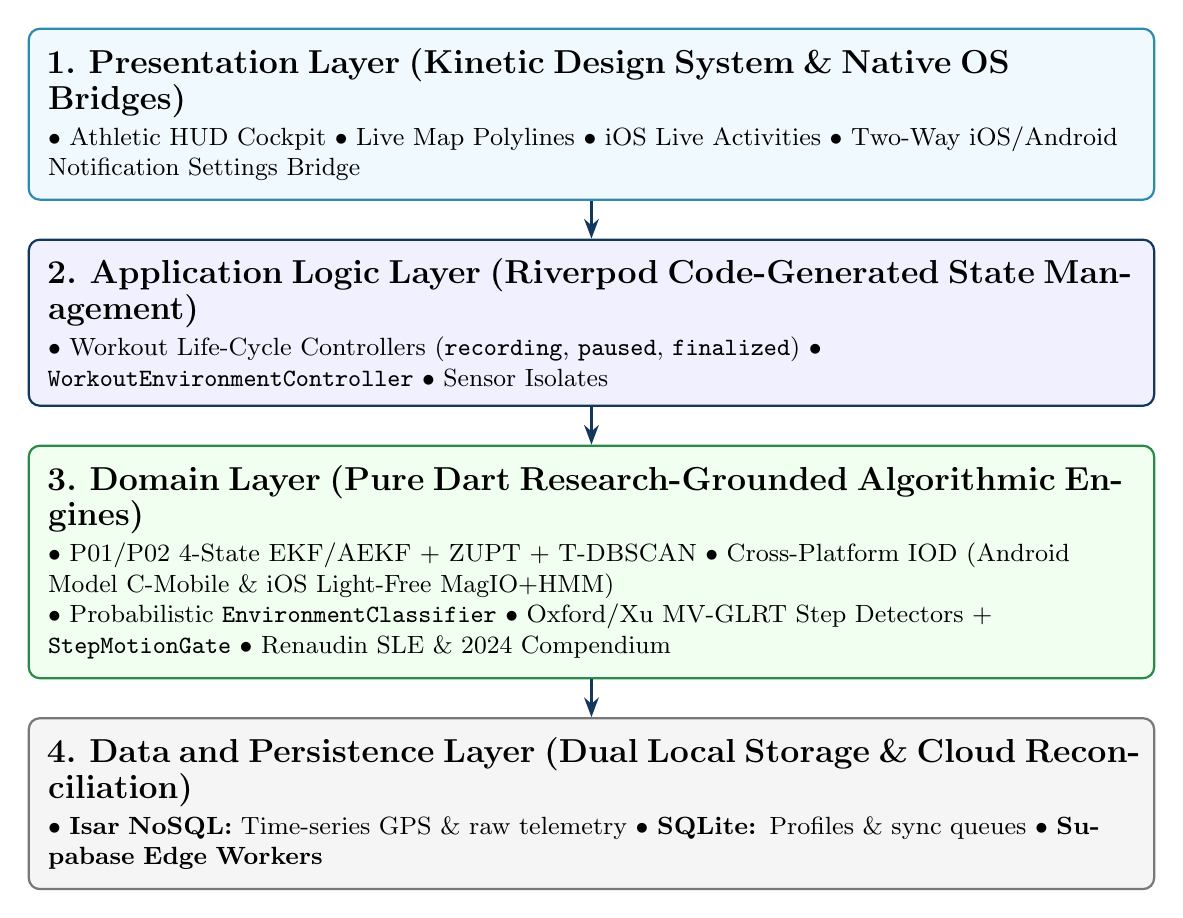
\begin{tikzpicture}[
    layer/.style={rectangle, draw=aetronblue, fill=blue!5, rounded corners=4pt, thick, text width=13.8cm, align=left, inner sep=7pt, font=\small},
    arrow/.style={-{Stealth[length=2.5mm]}, thick, color=aetronblue}
]
    % Layer 1: Presentation
    \node[layer, fill=cyan!6, draw=aetroncyan] (l1) {
        \textbf{\large 1. Presentation Layer (Kinetic Design System \& Native OS Bridges)}\\[2pt]
        $\bullet$ Athletic HUD Cockpit $\bullet$ Live Map Polylines $\bullet$ iOS Live Activities $\bullet$ Two-Way iOS/Android Notification Settings Bridge
    };

    % Layer 2: Application Logic
    \node[layer, fill=blue!6, draw=aetronblue, below=0.48cm of l1] (l2) {
        \textbf{\large 2. Application Logic Layer (Riverpod Code-Generated State Management)}\\[2pt]
        $\bullet$ Workout Life-Cycle Controllers (\texttt{recording}, \texttt{paused}, \texttt{finalized}) $\bullet$ \texttt{WorkoutEnvironmentController} $\bullet$ Sensor Isolates
    };

    % Layer 3: Domain
    \node[layer, fill=green!6, draw=codegreen, below=0.48cm of l2] (l3) {
        \textbf{\large 3. Domain Layer (Pure Dart Research-Grounded Algorithmic Engines)}\\[2pt]
        $\bullet$ P01/P02 4-State EKF/AEKF + ZUPT + T-DBSCAN $\bullet$ Cross-Platform IOD (Android Model~C-Mobile \& iOS Light-Free MagIO+HMM)\\
        $\bullet$ Probabilistic \texttt{EnvironmentClassifier} $\bullet$ Oxford/Xu MV-GLRT Step Detectors + \texttt{StepMotionGate} $\bullet$ Renaudin SLE \& 2024 Compendium
    };

    % Layer 4: Data Persistence
    \node[layer, fill=gray!8, draw=codegray, below=0.48cm of l3] (l4) {
        \textbf{\large 4. Data and Persistence Layer (Dual Local Storage \& Cloud Reconciliation)}\\[2pt]
        $\bullet$ \textbf{Isar NoSQL:} Time-series GPS \& raw telemetry $\bullet$ \textbf{SQLite:} Profiles \& sync queues $\bullet$ \textbf{Supabase Edge Workers}
    };

    % Connections
    \draw[arrow] (l1.south) -- (l2.north);
    \draw[arrow] (l2.south) -- (l3.north);
    \draw[arrow] (l3.south) -- (l4.north);
\end{tikzpicture}
\caption{Layered Architecture of the Aetron Mobile Fitness Tracking Platform.}
\label{fig:aetron_architecture}
\end{figure}

\begin{enumerate}
    \item \textbf{Presentation Layer (Kinetic Design System):} Delivers editorial-style athletic HUDs, live route recaps, iOS Live Activities, and direct native OS notification settings deep-linking (\path{UNUserNotificationCenter} / \path{openNotificationSettingsURLString} on iOS and \path{ACTION_APP_NOTIFICATION_SETTINGS} on Android). Experimental IOD overlays are removed from the production recording screen while background telemetry continues non-intrusively.
    \item \textbf{Application Logic Layer (Riverpod):} Implemented with \path{riverpod_annotation}~\cite{riverpod2024state}, coordinating workout life-cycles, background sensor streams, and environment controllers without blocking the UI thread.
    \item \textbf{Domain Layer (Pure Dart Algorithmic Services):} Houses all mathematical filtering, neural/probabilistic IOD, MV-GLRT step detection, stride estimation, and calorimetry engines in platform-independent pure Dart, enabling 100\% deterministic execution on headless CI runners.
    \item \textbf{Data and Persistence Layer:} Pairs \textbf{Isar NoSQL}~\cite{isar2024database} (high-throughput time-series GPS and workout logs) with \textbf{SQLite} (user profiles and sync queues) and \textbf{Supabase}~\cite{supabase2024backend} Deno edge workers (\texttt{deterministic-finalize-worker} and \texttt{route-correction-worker}) for canonical post-workout reconciliation.
\end{enumerate}

\section{Outdoor GPS Pipeline and Kinematic State Estimation}
\label{sec:gps_pipeline_design}
The outdoor tracking pipeline converts raw mobile location fixes into a smoothed, geodetically consistent trajectory.

\subsection{Planar Coordinate Projection and Phase~1 Preprocessing}
To avoid repeated spherical trigonometry inside the $1$\,Hz Kalman loop, Aetron projects incoming coordinates $(\phi, \lambda)$ onto a local Equirectangular tangent plane anchored at $(\phi_0, \lambda_0)$:
\begin{align}
    p_x &= R_{\text{earth}} \cdot (\lambda - \lambda_0) \cdot \cos\left(\frac{\phi_0 \cdot \pi}{180}\right) \cdot \frac{\pi}{180} \\
    p_y &= R_{\text{earth}} \cdot (\phi - \phi_0) \cdot \frac{\pi}{180}
\end{align}
Introducing $<0.01\%$ distortion for workout radii $<50$\,km, this representation enables closed-form matrix operations. Upstream Phase~1 preprocessing (\cite{zheng2015trajectory,li2025trajectory}) applies modality-specific speed/acceleration limits, sliding-window median outlier rejection, Zheng~\cite{zheng2009mining} stay-point detection, and outage segmentation before fixes enter the filter.

\subsection{4-State Kinematic EKF, Joseph Stabilization, and Phase~2 Gating}
Implemented in \texttt{ExtendedKalmanFilter} (\texttt{lib/features/workout/domain/services/ekf/}), the state vector $\mathbf{x} = [p_x, p_y, v, \theta]^T$ maintains local position, ground speed, and heading:
\begin{itemize}
    \item \textbf{Heading Phase Normalization \& Low-Speed Deadband:} Heading $\theta$ wraps continuously to $[0, 2\pi)$ with shortest-arc angular residuals; noisy GNSS course readings are suppressed below modality speed deadbands ($0.8 / 1.2 / 1.8$\,m/s for walk/run/cycle).
    \item \textbf{Joseph-Form Covariance Stabilizer:} Covariance $\mathbf{P}_k$ is updated exclusively via Equation~\ref{eq:joseph_form} on flat \texttt{Float64List} buffers with Cauchy--Schwarz off-diagonal clamping ($|P_{EN}| \le 0.99\sqrt{P_{EE}P_{NN}}$).
    \item \textbf{2-DOF Mahalanobis Gating \& Centripetal Scaling:} Under Phase~2 GNSS correction~\cite{groves2013principles,rongli2003survey}, spatial NIS $d_M^2 = \boldsymbol{\nu}_k^T \mathbf{S}_k^{-1} \boldsymbol{\nu}_k$ is compared against $\chi^2_2$ quantiles ($\gamma_1 = 5.991$, $\gamma_2 = 13.816$): moderate innovations inflate $\sigma_{\text{eff}} = \sigma_k \sqrt{d_M^2/\gamma_1}$, severe jumps ($d_M^2 > \gamma_2$) are rejected unless $N_{\text{reanchor}} = 4$ consecutive fixes confirm a genuine shift, and sharp turns scale heading process noise by $\mu_\theta = \min(\mu_{\max}, 1 + 0.8(\dot{\psi}_k/\omega_{\text{th}})^2)$.
    \item \textbf{Stationary ZUPT \& T-DBSCAN Dwell Clustering:} When $v < 0.3$\,m/s for $\ge 3$\,s, ZUPT clamps velocity to zero and scales $\mathbf{Q}_k$ by $0.01$. Complementarily, \texttt{GpsDbscanService}~\cite{ester1996dbscan} scans sequential low-speed fixes ($v_k \le 1.0$\,m/s), expanding a dwell cluster while $d_{\text{geo}}(\bar{\mathbf{c}}_{i:j-1}, p_j) \le \varepsilon = 6.5$\,m and confirming stationary stops when $\mathrm{MinPts} \ge 4$ and duration $\ge 10.0$\,s (collapsing courtyard dwell clouds to their centroid).
\end{itemize}

\section{Cross-Platform Indoor/Outdoor Detection Architecture}
\label{sec:deepiod_impl}
To provide seamless indoor--outdoor awareness across both Android and iOS despite asymmetric OS sensor sandboxing, \texttt{IodCompositeClassifier} routes incoming telemetry snapshots (\texttt{IodSensorSnapshot}) dynamically by verified hardware capability.

\subsection{Android Path: Unprivileged 4-Channel Model~C-Mobile \& Yoo $C/N_0$}
Because unprivileged background apps cannot query cellular RSRP/RSRQ used in full 8-channel DeepIOD~\cite{dastagir2024deepiod}, Android devices with an ambient light photodiode execute \textbf{Model~C-Mobile} (\path{lib/features/iod/domain/services/deepiod_neural_classifier.dart}), a pure-Dart 2D Depthwise Separable CNN over four unprivileged channels:
\begin{equation}
    \mathbf{X}_{\text{input}} \in \mathbb{R}^{B \times 4 \times W} = \left[\text{Light},\; \text{Mag},\; \text{Acc},\; \text{Daytime}\right]
\end{equation}
combining log-scaled illuminance $\log_{10}(1 + \text{lux})$, geomagnetic magnitude $\|\mathbf{m}\|$ and rolling variance, linear acceleration variance, and deterministic astronomical daytime. Its architecture executes:
\begin{enumerate}
    \item \textbf{Input Preprocessing Layer:} Population standardization ($\mu=0, \sigma=1$) over 10-second windows.
    \item \textbf{2D Depthwise Separable Convolution:} Channel-wise $3\times 3$ filtering followed by $1\times 1$ pointwise projection, cutting parameters by 78\%.
    \item \textbf{Batch Normalization and LeakyReLU Activation:} Folded statically into convolutional weights.
    \item \textbf{Global Average Pooling and Sigmoid Head:} Emits instantaneous $P(\text{Outdoor}) \in [0, 1]$ using only \textbf{54.0\,KB} of weights in $<0.8$\,ms per window without TFLite/ONNX native bloat.
\end{enumerate}
Where Android \texttt{GnssStatus} exposes satellite $C/N_0$, \texttt{SeamlessTransitionDetector} fuses Yoo's probabilistic $30$--$40$\,dB-Hz transition curve~\cite{yoo2025seamless}.

\subsection{iOS-First Light-Free Multi-Sensor Classifier}
On iOS, public APIs expose neither ambient light nor raw satellite $C/N_0$, causing light-dependent 4-channel models to abstain completely ($0\%$ coverage). We therefore engineered \texttt{IosMultiSensorIodClassifier} (\path{lib/features/iod/domain/services/ios_multisensor_iod_classifier.dart}) strictly from unprivileged cross-platform sensors (\texttt{CMMotionManager}, \texttt{CoreLocation}, and \texttt{CMAltimeter}):
\begin{enumerate}
    \item \textbf{MagIO Magnetic Perturbation Vector (Ashraf et al., 2018~\cite{ashraf2018magio}):} Over a causal 10-second sliding buffer of magnetic magnitude $\|\mathbf{m}_k\|$, the service computes 10 distributional features: mean, standard deviation, min, max, range, median, interquartile range (IQR), skewness, kurtosis, and mean absolute first derivative $|\Delta \|\mathbf{m}\||$.
    \item \textbf{Inertial Dynamics \& Diurnal Prior (Esmaeili Kelishomi et al., 2019~\cite{kelishomi2019activities}):} Appends 10-second linear acceleration mean, standard deviation, and peak-to-peak excursion alongside deterministic astronomical daytime, forming a 14-dimensional feature vector passed through a pure-Dart frozen 2-layer MLP trained exclusively on Cambridge CIOD Sessions~00--59 (threshold tuned on Validation Sessions~60--71).
    \item \textbf{CoreLocation \& Barometer Runtime Likelihood Fusion (Bui et al., 2020~\cite{bui2020gpsiod}; Li et al., 2014~\cite{li2014iodetector}; F{\'e}riol et al., 2020~\cite{feriol2020review}):} When live GNSS horizontal accuracy $\sigma_{\text{acc}}$, raw GPS fix silence age $\Delta t_{\text{silence}}$, or \texttt{CMAltimeter} 10-second pressure delta $\Delta P_{10\text{s}}$ (acquired via \texttt{IodSensorAcquisitionService}) are present, emission probability $b_t(\text{Out})$ combines the neural MagIO+Acc posterior with sigmoid CoreLocation accuracy/outage likelihoods and barometric doorway/elevator step evidence ($|\Delta P_{10\text{s}}| \ge 0.35$\,hPa) using IODetector confidence weighting~\cite{li2014iodetector}.
    \item \textbf{Causal 2-State HMM Forward Filter (Zhu et al., 2019~\cite{zhu2019fast}):} Frame emissions are smoothed recursively via Equation~\ref{eq:hmm_lit} with diagonal self-transition retention ($A_{ss} = 0.90$), preventing single-epoch urban-canyon flickers while responding to genuine building entries within $3$--$4$\,s.
\end{enumerate}

\subsection{Probabilistic \texttt{EnvironmentClassifier} with Path Straightness}
To eliminate legacy ad-hoc linear score weights ($0.45/0.30/0.15/0.10$) in the core workout tracker, \texttt{EnvironmentClassifier} (\path{lib/core/services/environment_detector.dart}) now computes calibrated sigmoid GNSS accuracy likelihoods~\cite{bui2020gpsiod,dastagir2024deepiod}, evaluates \textbf{Benhamou's (2004) Path Straightness Index}~\cite{benhamou2004tortuosity}:
\begin{equation}
    S = \frac{d_{\text{net}}}{\max(d_{\text{path}}, 1.0)} \in [0, 1]
    \label{eq:benhamou_s}
\end{equation}
over recent GPS trajectories to separate straight outdoor paths ($S \to 1$) from tortuous indoor multipath clouds ($S \to 0$), enforces an 8-second GPS-blackout + active-step indoor gate for iPhone gymnasiums, and filters posterior state through the same causal 2-state HMM~\cite{zhu2019fast}.

\section{Adaptive Transition Engine Architecture}
\label{sec:transition_engine_design}
To suppress boundary jitter on instantaneous neural outputs, Aetron encapsulates Model~C-Mobile within an \textbf{Adaptive Transition Engine} (\texttt{IndoorOutdoorTransitionEngine}), formalized in Algorithm~\ref{alg:transition_engine}.

\begin{algorithm}[htbp]
\KwIn{Sensor Snapshot $\mathbf{s}_t$, Previous State $S_{t-1}$, Hysteresis Thresholds $\theta_{\text{high}}=0.65, \theta_{\text{low}}=0.35$, Minimum Dwell Epochs $N_{\text{dwell}}=5$}
\KwOut{Committed State $S_t \in \{\text{Indoor}, \text{Outdoor}\}$, Uncertainty Flag $U_t$}

$P_t \leftarrow \text{ModelC\_Mobile}(\mathbf{s}_t)$\;
$U_t \leftarrow (P_t \ge 0.40 \land P_t \le 0.60)$ \tcp*{Epistemic uncertainty band}

\tcp{Schmitt Trigger Dual-Threshold Evaluation}
\eIf{$S_{t-1} == \text{Indoor}$}{
    \eIf{$P_t \ge \theta_{\text{high}}$}{
        $C_t \leftarrow \text{Outdoor}$ \tcp*{Candidate transition}
    }{
        $C_t \leftarrow \text{Indoor}$\;
    }
}{
    \eIf{$P_t \le \theta_{\text{low}}$}{
        $C_t \leftarrow \text{Indoor}$ \tcp*{Candidate transition}
    }{
        $C_t \leftarrow \text{Outdoor}$\;
    }
}

\tcp{Minimum Dwell-Time Debouncing State Machine}
\eIf{$C_t \ne S_{t-1}$}{
    \eIf{$C_t == \text{PendingState}_{t-1}$}{
        $\text{PendingDwell}_t \leftarrow \text{PendingDwell}_{t-1} + 1$\;
        \eIf{$\text{PendingDwell}_t \ge N_{\text{dwell}}$}{
            $S_t \leftarrow C_t$ \tcp*{Commit handover}
            $\text{Dwell}_t \leftarrow \text{PendingDwell}_t$\;
            $\text{PendingState}_t \leftarrow \text{None}$\;
            $\text{EmitHandoverEvent}(S_{t-1} \to S_t)$\;
        }{
            $S_t \leftarrow S_{t-1}$\;
            $\text{Dwell}_t \leftarrow \text{Dwell}_{t-1} + 1$\;
            $\text{PendingState}_t \leftarrow C_t$\;
        }
    }{
        $\text{PendingState}_t \leftarrow C_t$\;
        $\text{PendingDwell}_t \leftarrow 1$\;
        $S_t \leftarrow S_{t-1}$\;
        $\text{Dwell}_t \leftarrow \text{Dwell}_{t-1} + 1$\;
    }
}{
    $S_t \leftarrow S_{t-1}$\;
    $\text{Dwell}_t \leftarrow \text{Dwell}_{t-1} + 1$\;
    $\text{PendingState}_t \leftarrow \text{None}$\;
    $\text{PendingDwell}_t \leftarrow 0$\;
}
\Return{$(S_t, U_t)$}\;
\caption{Adaptive Transition Debouncing and Handover Algorithm}
\label{alg:transition_engine}
\end{algorithm}

The engine enforces Schmitt-trigger hysteresis ($\theta_{\text{high}} = 0.65, \theta_{\text{low}} = 0.35$), minimum persistence debouncing ($N_{\text{dwell}} = 5$\,s), and epistemic uncertainty flagging ($P_t \in [0.40, 0.60]$).

\section{Inertial Step Detection, MV-GLRT Gating, Cadence, and Stride Length}
\label{sec:cadence_engine_design}

\subsection{Causal Step Detectors with Skog MV-GLRT ZUPT and Bout Gating}
Alongside hardware pedometer adapters (\texttt{TYPE\_STEP\_COUNTER} / \texttt{CMPedometer} with reboot-safe baseline anchoring), Aetron implements two causal pure-Dart inertial detectors hardened against stationary false steps:
\begin{itemize}
    \item \textbf{Walking (\texttt{OxfordStepDetector}):} Adapts Salvi et al.~\cite{salvi2018oxford} ($100$\,Hz resampling, 13-tap Gaussian FIR, 35-sample midpoint prominence $s_k$, online Welford threshold $s_n - \mu_n > \max(1.2\sigma_n, 0.35)$, and causal $200$\,ms refractory confirmation so terminal steps are not dropped).
    \item \textbf{Running (\texttt{XuRunningStepDetector}):} Adapts Xu et al.~\cite{xu2022step} ($50$\,Hz resampling, 11-tap Hamming LPF at $5$\,Hz, 256-point real DFT dominant gait frequency extraction, and adaptive peak gating).
    \item \textbf{Skog et al. (2010) MV-GLRT Stance Rejection:} Replacing ad-hoc min-max amplitude spans vulnerable to single screen taps, both detectors evaluate Equation~\ref{eq:mv_glrt_lit} over a $1.0$\,s rolling magnitude window against Brajdic \& Harle-calibrated variance floors~\cite{skog2010zupt,brajdic2013walk}: $\gamma_{\text{MV}} = 0.36\text{ (m/s}^2)^2$ for walking ($\sigma \ge 0.60$\,m/s$^2$) and $\gamma_{\text{MV}} = 0.64\text{ (m/s}^2)^2$ for running ($\sigma \ge 0.80$\,m/s$^2$).
    \item \textbf{Rhythmic Bout \& GNSS Lock (\texttt{StepMotionGate}):} Grounded in Brajdic \& Harle~\cite{brajdic2013walk}, \texttt{StepMotionGate} buffers candidate steps until $N_{\text{bout}} = 5$ consecutive steps arrive within physiological gait cadence ($[0.65, 4.5]$\,Hz; inter-step gap $\le 2.2$\,s), and purges buffered in-place impulses whenever high-accuracy outdoor GNSS proves zero displacement past a $3.5$\,s onset grace window.
\end{itemize}

\subsection{6-Second Sliding-Window Cadence and Renaudin Adaptive Step Length}
\texttt{CadenceCalculatorService} resolves the Cadence Trilemma with a 6-second circular FIFO buffer and $4.0$\,s auto-decay inactivity timeout:
\begin{equation}
    \text{Cadence}_{\text{live}}(t) =
    \begin{cases}
        0 & \text{if } t - t_{\text{last\_step}} > 4.0\,\text{s} \text{ or } N_{\text{window}} < 2 \\
        \min\!\left(270, \frac{N_{\text{window}} \times 60}{6.0}\right) & \text{otherwise}
    \end{cases}
\end{equation}
For indoor or GPS-denied distance estimation, \texttt{ResearchStepLengthFallback} evaluates Renaudin et al.'s linear stature--frequency model (Equation~\ref{eq:renaudin_lit})~\cite{renaudin2012step} using LOSO-validated parameters: $(a, b, c) = (0.1328, 0.0217, 0.2755)$ for walking ($H \in [1.60, 1.88]$\,m, $C \in [94, 144]$\,spm) and $(0.3211, 0.7253, -1.6810)$ for running ($H \in [1.627, 1.872]$\,m, $C \in [143, 223]$\,spm), clamping safely to cohort means outside validated support rather than extrapolating unboundedly.

\section{Offline Trajectory Reconstruction, Compression, and Calorimetry}
\label{sec:reconstruction_design}

\subsection{Display-Only Outage Reconstruction and Polyline Compression}
Post-workout, \texttt{WorkoutSessionFinalizer} bridges short GNSS dropouts ($2.0\,\text{s} < \Delta t_{\text{gap}} \le 15.0\,\text{s}$) via either Linear Chord or Fritsch--Carlson Monotone PCHIP~\cite{fritsch1980pchip} (configured by \texttt{kTrajectoryReconstructionMethod}), while isolating blackouts $>15.0$\,s without fabrication. \textbf{Strict offline isolation} guarantees that zero synthetic points ever enter the live EKF, saved distance accumulator, or server segment audits. Before cloud synchronization, \texttt{PolylineCompressionService} applies Google Encoded Polyline delta quantization ($10^{-5}$ or $10^{-6}$\,deg), and \texttt{deterministic-finalize-worker} + \texttt{route-correction-worker} reconcile canonical server metrics (\texttt{METRICS\_VERSION = 2}), explicitly reporting \texttt{routeMatchingAvailable() = false} when no OSRM road-graph provider is attached~\cite{newson2009hidden}.

\subsection{2024 Adult Compendium Caloric Expenditure}
\label{sec:calorie_design}
Both the Flutter client (\path{UserProfile.calculateCalories}) and Supabase edge worker (\path{compendium_met.ts}) compute distance-activity kilocalories via Equation~\ref{eq:compendium_2024} using exact 5-digit speed-banded codes from the \textbf{2024 Adult Compendium of Physical Activities}~\cite{herrmann2024compendium} (walking \texttt{17151}--\texttt{17255}, running \texttt{12028}--\texttt{12145}, cycling \texttt{01010}--\texttt{01060}) converted via $v_{\text{mph}} = v_{\text{km/h}} / 1.609344$ without unverified interpolation across speed-band gaps, returning strictly $0$\,kcal whenever verified moving displacement is zero. Non-distance indoor activities (gym, yoga) fall back to duration-based MET integration with a $0.95$ female adjustment factor.

\section{System Safety, Feature Flags, and Observational Isolation}
\label{sec:safety_gating}
All research pipeline switches are governed by compile-time \texttt{--dart-define} constants in \texttt{lib/core/constants/debug\_config.dart}:
\begin{itemize}
    \item \texttt{kGpsFilterAlgoConfig = 'ekf4State'} (4-state kinematic EKF default; \texttt{fixedAlpha} preserved only for A/B replay).
    \item \texttt{kEnableTrajectoryPreprocessing = true} and \texttt{kEnableGnssCorrection = true} (Phase~1 kinematic preprocessing and Phase~2 Mahalanobis/turn-rate EKF guards).
    \item \texttt{kEnableTrajectoryReconstruction = true} (strictly offline display-only; never mutates distance or pace).
    \item \texttt{kEnableGpsQualityGate = false} (guarded behind explicit opt-in until further multi-device validation).
\end{itemize}
Crucially, every IOD classifier (\texttt{DeepIodNeuralClassifier}, \texttt{IosMultiSensorIodClassifier}, \texttt{IodCompositeClassifier}, \texttt{SeamlessTransitionDetector}) hardcodes \texttt{isObservationalOnly = true}. Experimental environment predictions are logged for scientific auditing without ever overriding the primary workout persistence state machine.

\chapter{Experiment Results and Evaluation}
\label{ch:evaluation}

\section{Evaluation Methodology and Field Contextualization}
Aetron was evaluated in two complementary tiers: (1)~\textbf{Smartphone Field Contextualization} carried forward from the pre-thesis evaluation~\cite{aetron2026prethesis} to verify real-world distance alignment against established commercial fitness apps and pre-measured urban routes; and (2)~\textbf{Reproducible Public-Dataset Benchmarking} executing both live runtime algorithms (EKF/AEKF, iOS light-free IOD, Model~C-Mobile, adapted MV-GLRT ZUPT, 6-second cadence, LOSO Renaudin stride, P03 reconstruction, and contiguous 2024 Compendium MET tables) and offline research comparators (sequential centroid-radius dwell clustering, linear-CV IGG-III/IAE, causal IMM/Zheng, and CAP-ALSTM + Python SHAP) on open public datasets with independent physical ground truth. Every offline experiment adheres strictly to an unbroken \textbf{Evidence Provenance Chain} summarized in Table~\ref{tab:evidence_chain}.

\begin{table}[htbp]
\centering
\caption{Complete Scientific Evidence Provenance Chain across All Evaluated Modules.}
\label{tab:evidence_chain}
\resizebox{\textwidth}{!}{
\begin{tabular}{@{}llllll@{}}
\toprule
\textbf{Module} & \textbf{Published Basis} & \textbf{Public Dataset} & \textbf{Ground Truth} & \textbf{Code / Benchmark Target} & \textbf{Primary Metrics} \\ \midrule
\textbf{1. Outdoor GNSS / EKF} & Groves~\cite{groves2013principles}; Sukhenko~\cite{sukhenko2025gnss}; & TU Wien RTK~\cite{tuwien2026gnss}; & Leica GS18 RTK; & \texttt{ExtendedKalmanFilter}; & Shared-mask RMSE, P95, \\
 & Rong Li~\cite{rongli2003survey}; Li~\cite{li2025trajectory} & SnapperGPS~2~\cite{beuchert2023snappergps} & u-blox ZED-F9P RTK & \texttt{run\_fixed\_alpha\_vs\_ekf.py} & Dist.\ Err., Cluster CI \\ \midrule
\textbf{2. Cross-Platform IOD} & Dastagir~\cite{dastagir2024deepiod}; Yoo~\cite{yoo2025seamless}; & Cambridge CIOD~\cite{bakirtzis2022ciod}; & Session-disjoint labels & \texttt{DeepIodNeuralClassifier}; & Acc, Macro-F1, In/Out Rec, \\
 & Ashraf~\cite{ashraf2018magio}; Zhu~\cite{zhu2019fast} & HAR-PMD~\cite{harpmd2025dataset} ($120$ subj.) & \& $46$ doorway transits & \texttt{IosMultiSensorIodClassifier} & Event F1, FT/hr, Delay \\ \midrule
\textbf{3. Step / MV-GLRT / Cad.} & Salvi~\cite{salvi2018oxford}; Xu~\cite{xu2022step}; & Oxford WPD; Xu G3; & Tally \& $60$\,fps video & \texttt{OxfordStepDetector}; & Count Acc, WAPE, False \\
 & Skog~\cite{skog2010zupt}; Brajdic~\cite{brajdic2013walk} & PedEval; OxWalk~\cite{oxwalk2022oxford} & ($119{,}572$ steps) & \texttt{StepMotionGate} / \texttt{Cadence} & Steps, MAE, Flutter, Lag \\ \midrule
\textbf{4. Adaptive Stride} & Renaudin~\cite{renaudin2012step}; & SLEDataset2~\cite{vezocnik2021sle} ($114$); & Optical MoCap \& & \texttt{ResearchStepLengthFallback} & Strict LOSO MAE (cm), \\
 & Fukuchi~\cite{fukuchi2017public} & Fukuchi RBDS ($84$ run) & Force-Plate Treadmill & \texttt{stride\_length\_benchmark\_test} & RMSE (cm), MAPE (\%) \\ \midrule
\textbf{5. Outage Reconst.} & Fritsch--Carlson~\cite{fritsch1980pchip}; & TU Wien ($10$ walks); & Held-out $5$\,s interior & \texttt{WorkoutSessionFinalizer} & Per-session \& Pooled \\
 & Czerwi{\'n}ski~\cite{czerwinski2026reconstruction} & SnapperGPS~2 ($12$ rides) & RTK coordinates & \texttt{replay\_tu\_wien\_p03\_closure.py} & RMSE, P95 (Display-Only) \\ \midrule
\textbf{6. Dwell \& Polyline} & Ester~\cite{ester1996dbscan}; Zheng~\cite{zheng2009mining}; & STAGA~\cite{spang2022staga} ($122{,}808$); & Mobility stop diary; & \texttt{GpsDbscanService}; & Stop Prec/F1, False Stops, \\
 & Herrmann~\cite{herrmann2024compendium} & $60$-min courtyard; $30{,}381$ pts & Stationary truth & \texttt{PolylineCompressionService} & Bytes Saved, MET Parity \\ \bottomrule
\end{tabular}
}
\end{table}

\section{Field Comparison with Commercial Reference Applications}
\label{sec:eval_commercial_field}
To contextualize Aetron against commercial applications in real outdoor conditions, six smartphones ran FITAPP, Goals-Fitness, Running by Adidas, Nike Run Club, Strava, and Aetron concurrently along the same urban park walking loop ($\approx 510$\,m, Route~B). Table~\ref{tab:commercial_route_b} and Figure~\ref{fig:route_b_comparison} show that Aetron recorded $0.52$\,km, squarely matching Strava ($0.52$\,km) within the $0.51$--$0.56$\,km commercial spread.

\begin{table}[htbp]
\centering
\caption{Recorded field metrics across six fitness applications on Route~B ($\approx 510$\,m urban walking loop; Strava summary screenshot omitted calories).}
\label{tab:commercial_route_b}
\resizebox{0.92\textwidth}{!}{
\begin{tabular}{@{}lcccc@{}}
\toprule
\textbf{Application} & \textbf{Duration} & \textbf{Distance (km)} & \textbf{Calories (kcal)} & \textbf{Avg Pace (min/km)} \\ \midrule
FITAPP & 08:06 & 0.51 & 44 & 15:58 \\
Goals-Fitness & 08:22 & 0.51 & 32 & 16:24 \\
Running (Adidas) & 07:57 & 0.56 & 32 & 14:08 \\
Nike Run Club & 08:09 & 0.51 & 28 & 15:47 \\
Strava & 08:16 & 0.52 & N/A & 15:54 \\
\textbf{Aetron (This Work)} & \textbf{08:21} & \textbf{0.52} & \textbf{34} & \textbf{16:03} \\ \bottomrule
\end{tabular}
}
\end{table}

\begin{figure}[htbp]
\centering
\begin{subfigure}[b]{0.31\textwidth}
    \centering
    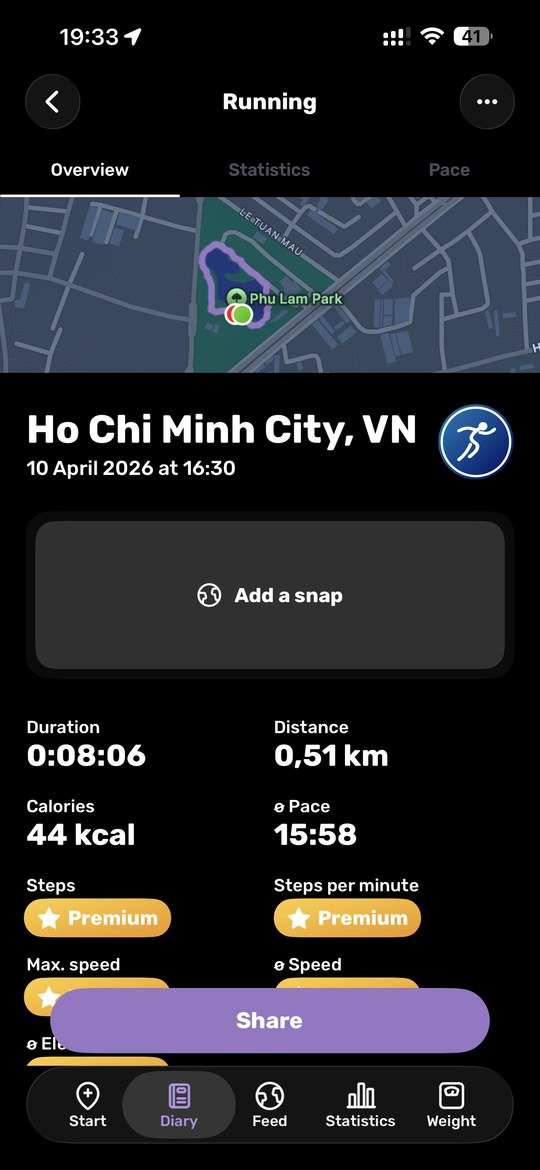
\includegraphics[height=5.2cm]{figures/cmp_fitapp.jpg}
    \caption{FITAPP ($0.51$\,km)}
\end{subfigure}\hfill
\begin{subfigure}[b]{0.31\textwidth}
    \centering
    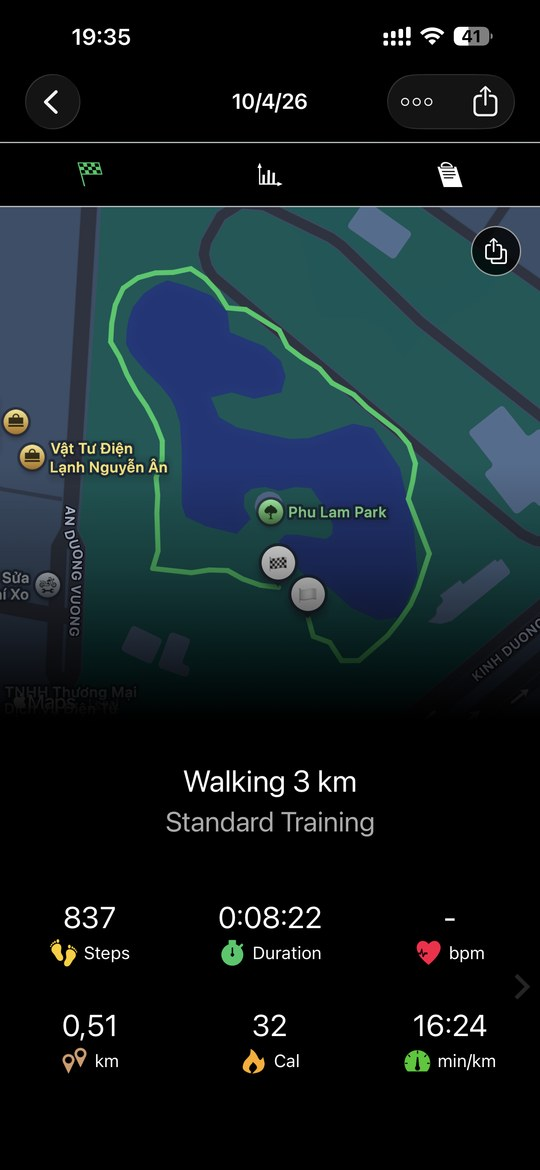
\includegraphics[height=5.2cm]{figures/cmp_goals.jpg}
    \caption{Goals-Fitness ($0.51$\,km)}
\end{subfigure}\hfill
\begin{subfigure}[b]{0.31\textwidth}
    \centering
    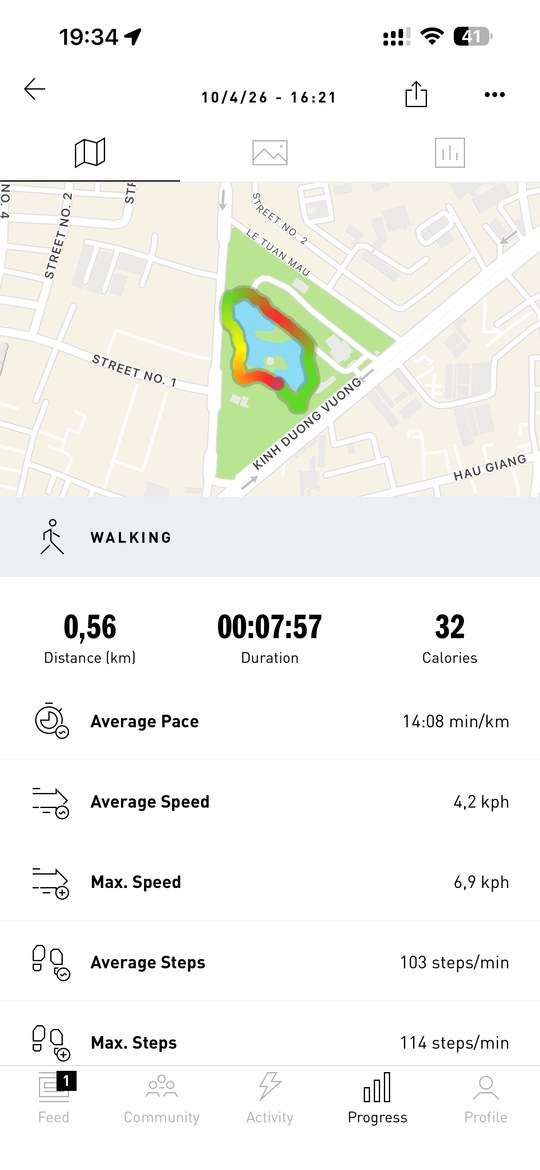
\includegraphics[height=5.2cm]{figures/cmp_adidas.jpg}
    \caption{Adidas Running ($0.56$\,km)}
\end{subfigure}\\[0.35cm]
\begin{subfigure}[b]{0.31\textwidth}
    \centering
    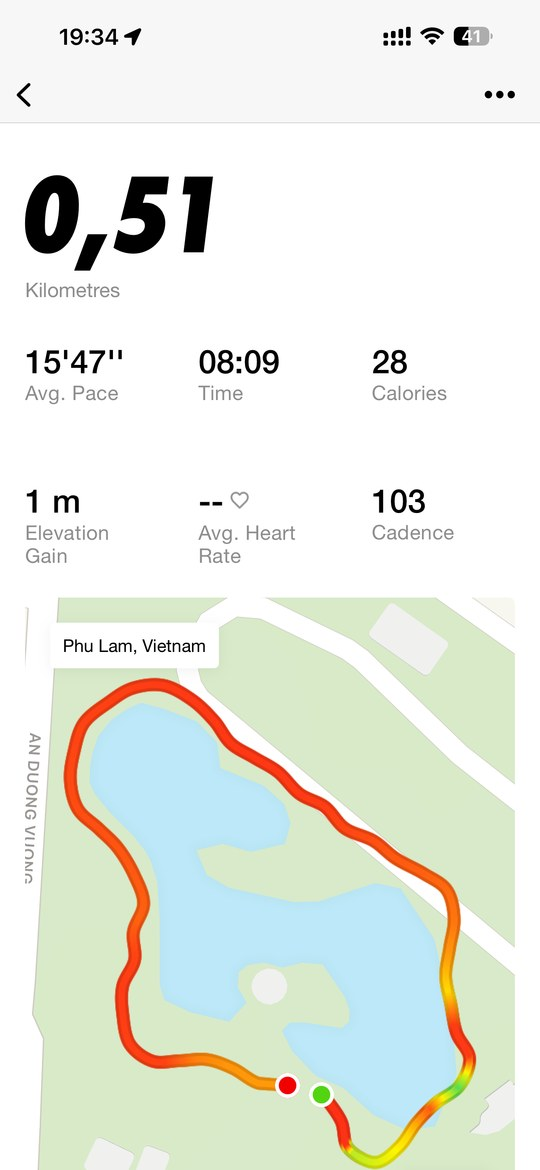
\includegraphics[height=5.2cm]{figures/cmp_nrc.jpg}
    \caption{Nike Run Club ($0.51$\,km)}
\end{subfigure}\hfill
\begin{subfigure}[b]{0.31\textwidth}
    \centering
    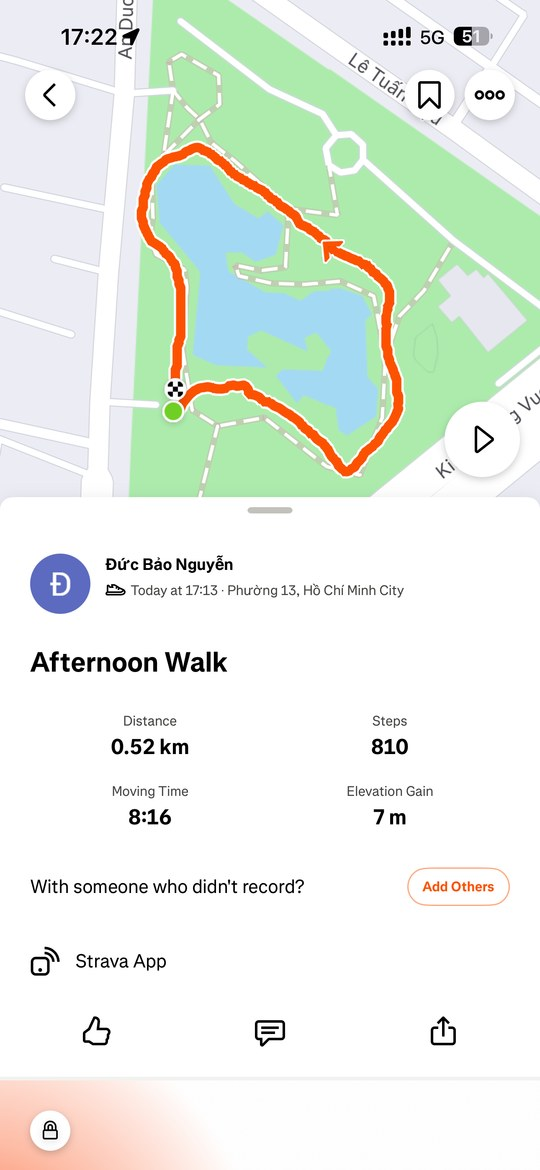
\includegraphics[height=5.2cm]{figures/cmp_strava.jpg}
    \caption{Strava ($0.52$\,km)}
\end{subfigure}\hfill
\begin{subfigure}[b]{0.31\textwidth}
    \centering
    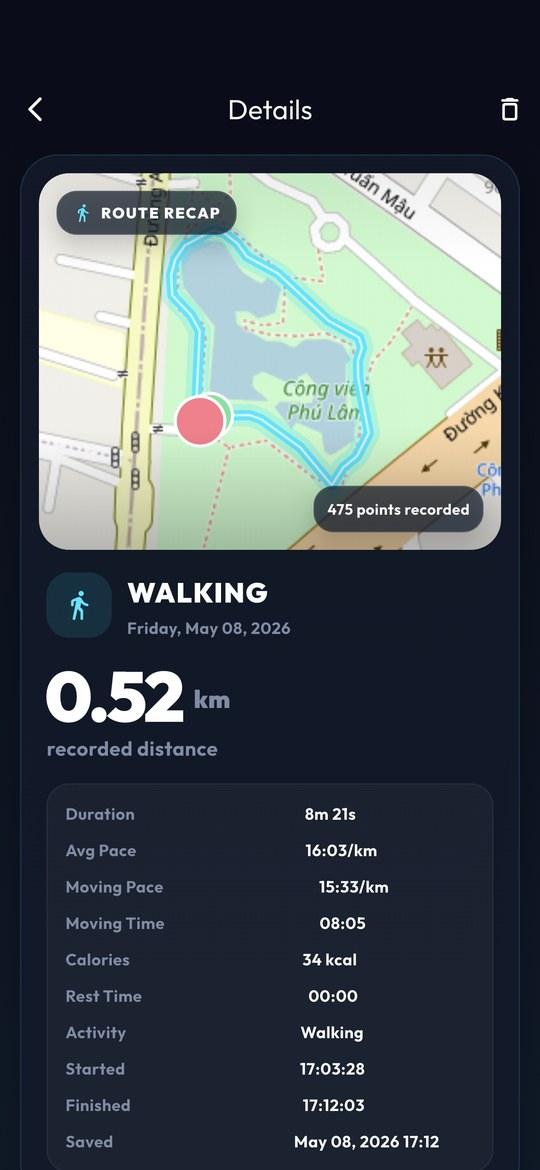
\includegraphics[height=5.2cm]{figures/cmp_aetron.jpg}
    \caption{Aetron ($0.52$\,km)}
\end{subfigure}
\caption{Route visualisation and recorded summary comparison across five commercial reference applications and Aetron on the same approximately $510$\,m outdoor walking route.}
\label{fig:route_b_comparison}
\end{figure}

\subsection{Initial Outdoor Field MAPE Benchmark (\texorpdfstring{$800$\,m}{800 m} Route)}
Following Tierney and Clarke~\cite{tierney2019gps} and Scott et al.~\cite{scott2016validity} ($\text{MAPE} = \frac{1}{N}\sum_{i=1}^{N}\left|\frac{d_i - d_{\text{ref}}}{d_{\text{ref}}}\right|\times 100\%$), an outdoor field trial over an $800$\,m reference corridor ($d_{\text{ref}} = 0.80$\,km on Google Maps, Figure~\ref{fig:mape_800m}) yielded $d_1 = 0.82$\,km, corresponding to an absolute error of $0.02$\,km and a \textbf{MAPE of 2.5\%}---well within Scott et al.'s $<5\%$ \textbf{Good} category and consistent with dedicated GNSS sports watches ($3.2$--$6.1\%$)~\cite{gilgenammann2020wrist}. Because consumer web-map baselines lack surveyed decimeter truth, Sections~\ref{sec:eval_gps_aekf}--\ref{sec:eval_calorie_drift} establish rigorous holdout evaluations against surveyor-grade RTK and optical motion capture datasets.

\begin{figure}[htbp]
\centering
\begin{subfigure}[t]{0.42\textwidth}
    \centering
    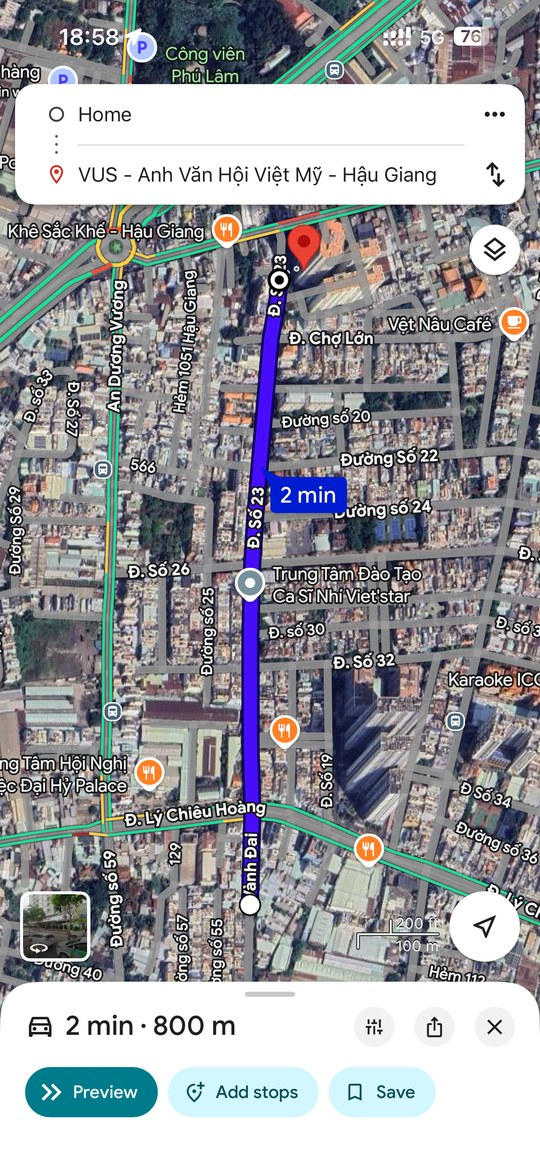
\includegraphics[height=6.2cm]{figures/mape_google_maps.jpg}
    \caption{Google Maps ($0.80$\,km)}
\end{subfigure}\hspace{0.8cm}
\begin{subfigure}[t]{0.42\textwidth}
    \centering
    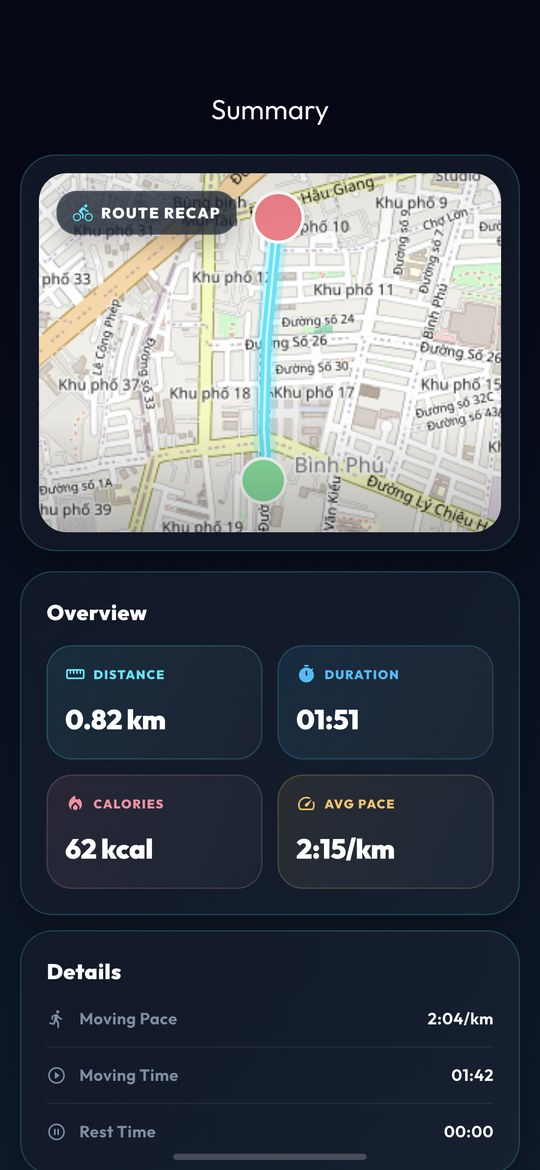
\includegraphics[height=6.2cm]{figures/mape_aetron.jpg}
    \caption{Aetron ($0.82$\,km, MAPE $2.5\%$)}
\end{subfigure}
\caption{Field MAPE benchmark validation comparing the pre-measured $800$\,m urban reference route against Aetron's recorded distance.}
\label{fig:mape_800m}
\end{figure}

\section{Outdoor GNSS Filtering, EKF vs.\ AEKF Audit, and Negative Results}
\label{sec:eval_gps_aekf}
In the TU~Wien Multi-GNSS dataset~\cite{tuwien2026gnss}, Google Pixel~9a, Pixel~7~Pro, and a Leica GS18 dual-frequency RTK antenna ($99.70\%$ fixed integer phase resolution, $CQ_{2D}\le 29.7$\,cm across the $1{,}680$-epoch Gate~3 cohort) were rigidly co-located on a collinear test stand across five physical walking routes in Vienna (Datasets~31--35). Timestamps were aligned to UTC and scored strictly on shared common epoch masks so outlier trimming could not bias RMSE.

\subsection{Isolated EKF vs.\ AEKF Ablation (Gate~3 NO-GO)}
Table~\ref{tab:tu_wien_gps_benchmark} tests whether adding isolated NIS covariance inflation ($\max(1.0, \text{NIS}_k / 5.991)$) over a calibrated 4-state EKF achieves our predefined $\ge 10\%$ RMSE acceptance gate. Across 10 recordings ($1{,}680$ epochs), isolated NIS scaling improved RMSE by only \textbf{+0.21\%} ($3.313$\,m $\to 3.306$\,m) with a paired 5-route cluster bootstrap 95\% CI of $[-0.0233, +0.0034]$\,m spanning zero, and slightly worsened Pixel~7~Pro accuracy ($-0.07\%$). Isolated NIS scaling alone therefore received a principled \textbf{NO-GO} verdict.

\begin{table}[htbp]
\centering
\caption{Isolated Gate~3 GNSS Filtering Benchmark on TU Wien Dataset vs.\ Leica GS18 RTK Truth ($1{,}680$ Epochs).}
\label{tab:tu_wien_gps_benchmark}
\resizebox{\textwidth}{!}{
\begin{tabular}{@{}lcccccccc@{}}
\toprule
\multirow{2}{*}{\textbf{Cohort / Device}} & \multicolumn{3}{c}{\textbf{Horizontal Position RMSE (m)}} & \multicolumn{2}{c}{\textbf{Error Percentiles (m)}} & \multicolumn{2}{c}{\textbf{AEKF vs.\ EKF}} & \multirow{2}{*}{\textbf{Gate Verdict}} \\ \cmidrule(lr){2-4} \cmidrule(lr){5-6} \cmidrule(lr){7-8}
 & \textbf{Raw (A)} & \textbf{EKF (B)} & \textbf{AEKF (D)} & \textbf{P50} & \textbf{P95} & \textbf{$\Delta$ RMSE} & \textbf{95\% Cluster CI} & \\ \midrule
Pixel 9a Aggregate ($N=5$ routes) & 2.852 & 2.022 & 2.005 & 1.65 & 3.81 & +0.84\% & $[-0.0467, +0.0002]$\,m & FAIL ($<10\%$) \\
Pixel 7 Pro Aggregate ($N=5$ routes) & 5.141 & 4.604 & 4.608 & 3.92 & 8.86 & -0.07\% & $[-0.0035, +0.0108]$\,m & FAIL ($<10\%$) \\ \midrule
\textbf{Total Combined Cohort} & \textbf{3.996} & \textbf{3.313} & \textbf{3.306} & \textbf{2.78} & \textbf{6.34} & \textbf{+0.21\%} & $\mathbf{[-0.0233, +0.0034]}$\,\textbf{m} & \textbf{OVERALL NO-GO} \\ \bottomrule
\end{tabular}
}
\end{table}

\subsection{Pre-Thesis Fixed-Alpha vs.\ 4-State EKF and Full \texttt{P01+P02} Production Replay}
Across all $3{,}286$ matched TU~Wien epochs (Table~\ref{tab:fixed_alpha_vs_ekf_benchmark}), Standard 4-state EKF cuts RMSE by \textbf{5.97\%} over pure Fixed-Alpha blending ($3.560$\,m vs.\ $3.789$\,m) and by \textbf{46.64\%} over Pre-Thesis Fixed-Alpha Full ($6.722$\,m), whose greedy stationary freeze collapsed during $1$\,Hz walking strides. Furthermore, evaluating Aetron's full production Dart pipeline (\texttt{P01} preprocessing + \texttt{P02} Mahalanobis gating + turn-rate scaling) on $2{,}694$ common phase-RTK epochs (Table~\ref{tab:gnss_p01_p02_snapper}) resolves legacy marker freeze ($8.753$\,m Fixed-Alpha and $10.181$\,m Legacy EKF $\to \mathbf{3.432}$\,m RMSE, $-60.8\%$) and reduces contiguous distance error to \textbf{1.34\%} (well within Scott et al.'s $<5\%$ \textbf{Good} criterion).

Crucially, however, replaying all 12 Oxford SnapperGPS~2 cycling rides ($20{,}770$ epochs vs.\ u-blox ZED-F9P RTK~\cite{beuchert2023snappergps}) exposes a vital \textbf{negative result}: because SnapperGPS~2 lacks Doppler speed/course and emits CEP50 ($50\%$ radial confidence) rather than native OS $1\sigma$ radii, Phase~2 NIS gating rejects $75.36\%$ of fixes during fast cycling, inflating RMSE to $138.226$\,m. Preserving this failure delineates the exact sensor-contract boundaries required for safe AEKF deployment.

\begin{table}[htbp]
\centering
\caption{Head-to-Head Estimator Replay on TU Wien ($3{,}286$ Matched Epochs, $\sigma_{\text{acc}}=\max(2.5, \text{HDOP}\cdot 4)$).}
\label{tab:fixed_alpha_vs_ekf_benchmark}
\resizebox{\textwidth}{!}{
\begin{tabular}{@{}lccccccc@{}}
\toprule
\textbf{Pipeline Variant} & \textbf{RMSE (m)} & \textbf{MAE (m)} & \textbf{P50 (m)} & \textbf{P95 (m)} & \textbf{Dist.\ Err.\ (\%)} & \textbf{Stat.\ Drift (m)} & \textbf{Host CPU ($\mu$s)} \\ \midrule
1. Raw GNSS (Unfiltered) & 3.478 & 2.914 & 2.457 & 6.523 & 3.03\% & 128.09 & 0.00 \\
2. Fixed-Alpha Pure ($\alpha\in\{0.34,0.52,0.72\}$) & 3.789 & 3.186 & 2.697 & 7.044 & \textbf{1.42\%} & 110.57 & 17.20 \\
3. Pre-Thesis Fixed-Alpha Full & 6.722 & 5.470 & 4.783 & 11.897 & 7.03\% & \textbf{61.67} & 23.35 \\
4. Standard Linear KF (4-State CV) & \textbf{3.505} & \textbf{2.939} & \textbf{2.496} & \textbf{6.560} & 2.32\% & 124.50 & \textbf{5.92} \\
5. Standard EKF (4-State Kinematic) & 3.560 & 2.994 & 2.518 & 6.660 & 2.37\% & 132.46 & 22.57 \\ \bottomrule
\end{tabular}
}
\end{table}

\begin{table}[htbp]
\centering
\caption{Integrated Production \texttt{P01+P02} Benchmark on TU Wien Walks and SnapperGPS~2 Cycling.}
\label{tab:gnss_p01_p02_snapper}
\resizebox{\textwidth}{!}{
\begin{tabular}{@{}llrrrrrr@{}}
\toprule
\textbf{Dataset \& Ground Truth} & \textbf{Pipeline Variant} & \textbf{Common $N$} & \textbf{RMSE (m)} & \textbf{MAE (m)} & \textbf{P95 (m)} & \textbf{Adj.\ Dist.\ Err.\ (\%)} \\ \midrule
\multirow{4}{*}{TU Wien RTK~\cite{tuwien2026gnss} (Walk)}
 & Raw Smartphone GNSS & 2,694 & \textbf{2.113} & \textbf{1.886} & \textbf{3.429} & 4.15\% \\
 & Historical \texttt{Fixed Alpha} & 2,694 & 8.753 & 6.131 & 19.678 & 9.77\% \\
 & Aetron Legacy 4-State EKF (No P02) & 2,694 & 10.181 & 7.400 & 21.854 & 11.55\% \\
 & \textbf{Production \texttt{P01 + P02 (4-State AEKF)}} & \textbf{2,694} & \textbf{3.432} & \textbf{2.514} & \textbf{4.746} & \textbf{1.34\%} \\ \midrule
\multirow{4}{*}{SnapperGPS~2~\cite{beuchert2023snappergps} (Cycling$^\dagger$)}
 & Raw Snapshot Fixes & 20,770 & \textbf{27.670} & \textbf{18.380} & \textbf{46.462} & 360.34\% \\
 & Historical \texttt{Fixed Alpha} & 20,770 & 40.419 & 23.928 & 81.172 & 44.50\% \\
 & \texttt{P01 + Legacy 4-State EKF} & 20,770 & 64.337 & 33.697 & 137.303 & \textbf{13.41\%} \\
 & \texttt{P01 + P02 (4-State AEKF)} \textit{(Neg.\ Result)} & 20,770 & 138.226 & 63.778 & 373.104 & 15.18\% \\ \bottomrule
\end{tabular}
}
\vspace{0.1cm}
\parbox{\textwidth}{\footnotesize $^\dagger$Low-cost snapshot logger lacking Doppler velocity and emitting CEP50 rather than OS $1\sigma$ horizontal accuracy.}
\end{table}

\section{Cross-Platform Indoor/Outdoor Detection Evaluation}
\label{sec:eval_iod_benchmark}
Evaluating strict session-disjoint generalization on Cambridge CIOD~\cite{bakirtzis2022ciod} (Train Sessions~00--59, Validation~60--71, Held-Out Test Sessions~72--84, $N = 201{,}731$ epochs; Table~\ref{tab:ciod_ios_benchmark}) shows why a light-free multi-sensor pipeline is essential: Android's 4-channel Model~C-Mobile ($73.64\%$ Acc / $69.59\%$ Macro-F1) achieves $0\%$ coverage on Apple iOS. Our light-free \textbf{iOS \texttt{[MagIO+Acc+Daytime]} MLP} restores \textbf{100\% iOS coverage} while surpassing the 4-channel Android model (\textbf{77.07\% Acc}, \textbf{74.97\% Macro-F1}), and pairing it with Zhu et al.'s~\cite{zhu2019fast} causal 2-state HMM elevates Outdoor Recall from $45.28\%$ to \textbf{69.48\%} ($74.77\%$ Macro-F1) with zero lookahead lag. A $15.2$\,pp gap below the privileged 8-channel DeepIOD oracle ($90.17\%$) reflects missing cellular radio/sound channels.

At actual doorway boundaries ($46$ transitions over $56.04$\,hours, Table~\ref{tab:ciod_comprehensive_benchmark}), wrapping Model~C-Mobile in the Adaptive Transition Engine slashes false transitions by \textbf{78.22\%} ($51.04 \to 11.12$\,FT/hr), yet event F1 reaches only $4.39\%$ ($15/46$ transits matched). Furthermore, an external 120-participant audit on HAR-PMD~\cite{harpmd2025dataset} ($40$ phone models, $288{,}466$ epochs) revealed that DeepIOD Model~C-Mobile falls to \textbf{55.36\% Macro-F1} ($0.0\%$ indoor walking recall vs.\ $24.4\%$ outdoor rest recall) due to locomotion confounding. Consequently, keeping \texttt{isObservationalOnly = true} in production is empirically justified.

\begin{table}[htbp]
\centering
\caption{Session-Isolated Held-Out IOD Benchmark on Cambridge CIOD (Sessions~72--84, $N = 201{,}731$ Epochs).}
\label{tab:ciod_ios_benchmark}
\resizebox{\textwidth}{!}{
\begin{tabular}{@{}lccccc@{}}
\toprule
\textbf{Model Variant \& Sensor Profile} & \textbf{iOS Coverage} & \textbf{Accuracy (\%)} & \textbf{Macro-F1 (\%)} & \textbf{Indoor Rec.\ (\%)} & \textbf{Outdoor Rec.\ (\%)} \\ \midrule
Always-Indoor Baseline & 100\% & 58.97\% & 37.10\% & 100.00\% & 0.00\% \\
DeepIOD 8-Ch Research Oracle~\cite{dastagir2024deepiod} & 0\% (Privileged) & \textbf{90.59\%} & \textbf{90.17\%} & \textbf{94.33\%} & \textbf{85.21\%} \\ \midrule
Model~C-Mobile (4-Ch Android: Light+Mag+Acc+Day) & 0\% (No ALS) & 73.64\% & 69.59\% & 93.37\% & 45.28\% \\
MagIO GNB + Causal HMM (Mag-Only~\cite{ashraf2018magio,zhu2019fast}) & 100\% & 73.38\% & 70.67\% & 87.98\% & 52.40\% \\
\textbf{iOS [MagIO+Acc+Daytime] MLP (Raw)} & \textbf{100\%} & \textbf{77.07\%} & \textbf{74.97\%} & 89.94\% & 58.57\% \\
\textbf{iOS [MagIO+Acc+Daytime] MLP + Causal HMM} & \textbf{100\%} & 75.65\% & 74.77\% & 79.94\% & \textbf{69.48\%} \\ \bottomrule
\end{tabular}
}
\end{table}

\begin{table}[htbp]
\centering
\caption{Epoch-Level vs.\ Doorway Transition Detection on Cambridge CIOD ($46$ Ground-Truth Transits, $56.04$\,h).}
\label{tab:ciod_comprehensive_benchmark}
\resizebox{\textwidth}{!}{
\begin{tabular}{@{}lccccccc@{}}
\toprule
\textbf{Smoothing Policy} & \textbf{Epoch Acc} & \textbf{Macro-F1} & \textbf{Total Det.} & \textbf{Matched GT} & \textbf{Trans.\ Prec.} & \textbf{Event F1} & \textbf{FT / Hour} \\ \midrule
1. Raw Binary ($\theta=0.50$) & 73.64\% & 69.60\% & 2,890 & \textbf{30 / 46} & 1.04\% & 2.04\% & 51.04 / hr \\
2. Majority Vote ($W=7$) & 73.73\% & 69.70\% & 1,464 & 23 / 46 & 1.57\% & 3.05\% & 25.72 / hr \\
3. Dual Hysteresis ($[0.65, 0.35]$) & 73.97\% & 70.00\% & 1,042 & 21 / 46 & 2.02\% & 3.86\% & 18.22 / hr \\
4. Probabilistic EMA ($\alpha=0.30$) & 74.22\% & 70.16\% & 689 & 15 / 46 & 2.18\% & 4.08\% & 12.03 / hr \\
\textbf{5. Adaptive Engine (Debounced)} & \textbf{74.26\%} & \textbf{70.22\%} & \textbf{638} & 15 / 46 & \textbf{2.35\%} & \textbf{4.39\%} & \textbf{11.12 / hr} \\ \bottomrule
\end{tabular}
}
\end{table}

\section{Indoor Step Counting, MV-GLRT, Cadence, and Stride Length}
\label{sec:eval_cadence_benchmark}
Baseline manual-count hardware trials over five $100$-step indoor corridor walks~\cite{aetron2026prethesis} yielded $98.2 \pm 3.8$ reported steps ($3.0\% \pm 2.7\%$ mean error, Table~\ref{tab:manual_step_trials}), comfortably within the $5\%$ acceptance target.

Expanding to causal accelerometry datasets (Table~\ref{tab:step_mvglrt_benchmark}), \texttt{OxfordStepDetector} with Skog MV-GLRT ($\gamma_{\text{MV}}=0.36\text{ (m/s}^2)^2$) improved step agreement toward truth ($4{,}225$ vs.\ $4{,}236$ against $4{,}107$ GT steps on Oxford WPD~\cite{salvi2018oxford}), \texttt{XuRunningStepDetector} achieved \textbf{98.69\%} accuracy ($1.17\%$ WAPE, $2.02$\,spm MAE; MV-GLRT $1{,}265/1{,}280$ steps) on Xu Group~3~\cite{xu2022step}, and MV-GLRT ZUPT + \texttt{StepMotionGate} eliminated \textbf{100\%} of false steps during $60$\,s hand-sway and $2.2$\,m/s$^2$ 50\,ms screen taps.

Across 129 video-annotated sessions ($54.39$\,hours, $119{,}572$ steps) from PedEval~\cite{mattfeld2021pedeval} and OxWalk~\cite{oxwalk2022oxford} (Table~\ref{tab:cadence_trilemma_matrix}), our $6$-second cadence window cuts visual flutter by \textbf{50.0\%} ($5.68 \to 2.84$\,spm/s) while keeping steady-state MAE at \textbf{8.41\,spm} and pause/resume drift at $0.00\%$. Finally, strict LOSO cross-validation of Renaudin Eq.~8~\cite{renaudin2012step} (Table~\ref{tab:stride_loso_benchmark}) reduces walking stride MAE from $9.51$ to \textbf{8.61\,cm} on \texttt{SLEDataset2}~\cite{vezocnik2021sle} and running MAE from $20.42$ to \textbf{17.80\,cm} on Fukuchi RBDS~\cite{fukuchi2017public}.

\begin{table}[htbp]
\centering
\caption{Baseline indoor hardware step-counting accuracy over five $100$-step corridor trials~\cite{aetron2026prethesis}.}
\label{tab:manual_step_trials}
\begin{tabular}{@{}ccccccccc@{}}
\toprule
\textbf{Metric} & \textbf{Trial 1} & \textbf{Trial 2} & \textbf{Trial 3} & \textbf{Trial 4} & \textbf{Trial 5} & \textbf{Mean} & \textbf{Std Dev} \\ \midrule
App Steps & 93 & 103 & 99 & 100 & 96 & \textbf{98.2} & 3.8 \\
Error (\%) & 7.0\% & 3.0\% & 1.0\% & 0.0\% & 4.0\% & \textbf{3.0\%} & 2.7\% \\ \bottomrule
\end{tabular}
\end{table}

\begin{table}[htbp]
\centering
\caption{Causal Step Counting \& Stationary False-Step Rejection (Oxford WPD, Xu Group~3, Adversarial Suite).}
\label{tab:step_mvglrt_benchmark}
\resizebox{\textwidth}{!}{
\begin{tabular}{@{}llccc@{}}
\toprule
\textbf{Dataset / Stress Protocol} & \textbf{Detector Configuration} & \textbf{Sessions / GT Steps} & \textbf{Predicted Steps} & \textbf{Count Acc.\ / WAPE} \\ \midrule
Oxford WPD~\cite{salvi2018oxford} (Walking) & Aetron \texttt{OxfordStepDetector} (MV-GLRT $\gamma=0.36$) & 12 / 4,107 & 4,225 (vs.\ 4,236 span) & $93.16\%$ span acc; HW subset $97.69\%$ \\
Xu Group~3~\cite{xu2022step} (Running) & Aetron \texttt{XuRunningStepDetector} (Span / MV-GLRT) & 5 / 1,280 & 1,279 / 1,265 & \textbf{98.69\% / 1.17\%} ($2.02$\,spm MAE) \\
Stationary Adversarial Suite & 60\,s Hand-Sway ($\pm 0.4$\,m/s$^2$) \& $2.2$\,m/s$^2$ Screen Taps & 2 / 0 & \textbf{0} & \textbf{100\% Rejected} (MV-GLRT $<$ $\gamma_{\text{MV}}$) \\ \bottomrule
\end{tabular}
}
\end{table}

\begin{table}[htbp]
\centering
\caption{Cadence Multi-Cohort Matrix across Sliding Windows ($129$ Sessions, $119{,}572$ Ground-Truth Steps).}
\label{tab:cadence_trilemma_matrix}
\resizebox{\textwidth}{!}{
\begin{tabular}{@{}lccc@{}}
\toprule
\textbf{Evaluation Dimension \& Cohort} & \textbf{3-Second} & \textbf{6-Second (Aetron)} & \textbf{10-Second} \\ \midrule
PedEval Regular Walking MAE ($30$ sess., $31{,}435$ steps) & 10.75\,spm & \textbf{8.41\,spm} & 7.95\,spm \\
OxWalk Continuous Walking P13 MAE ($39$\,min, $4{,}064$ steps) & 8.48\,spm & \textbf{8.52\,spm} & 9.38\,spm \\
PedEval Aggregate Cohort MAE ($90$ sess., $56{,}668$ steps) & 19.89\,spm & 20.94\,spm & 25.00\,spm \\
Display Flutter in Regular Walking (spm/s) & $5.68 \pm 9.79$ & $\mathbf{2.84 \pm 6.19}$ \textbf{(-50.0\%)} & $1.67 \pm 5.18$ \\
True Stop Decay / Max Observed Transition Lag & 1.00\,s / 1.00\,s & \textbf{3.0--4.0\,s / 4.52\,s} & 4.0--5.0\,s / 5.93\,s \\ \bottomrule
\end{tabular}
}
\end{table}

\begin{table}[htbp]
\centering
\caption{Strict Leave-One-Subject-Out (LOSO) Step-Length Benchmark (SLEDataset2 \& Fukuchi RBDS).}
\label{tab:stride_loso_benchmark}
\resizebox{\textwidth}{!}{
\begin{tabular}{@{}llrrr@{}}
\toprule
\textbf{Cohort ($N$ Sessions)} & \textbf{Estimator (Strict LOSO)} & \textbf{MAE (cm)} & \textbf{RMSE (cm)} & \textbf{MAPE (\%)} \\ \midrule
\multirow{3}{*}{Walking ($114$ sessions)}
 & Legacy Static ($0.415 H$) & 9.51 & 11.73 & 12.99\% \\
 & \textbf{Renaudin Eq.~8 LOSO}~\cite{renaudin2012step} & \textbf{8.61} & \textbf{10.88} & \textbf{12.01\%} \\
 & Cohort Fallback (Known $H$ / Missing $H$) & 9.05 / 9.23 & 11.16 / 11.09 & 12.73\% / 12.92\% \\ \midrule
\multirow{3}{*}{Running ($84$ trials)}
 & Legacy Static ($0.65 H$) & 20.42 & 23.65 & 17.30\% \\
 & \textbf{Renaudin Eq.~8 LOSO}~\cite{renaudin2012step} & \textbf{17.80} & \textbf{20.94} & \textbf{15.29\%} \\
 & Cohort Fallback (Known $H$ / Missing $H$) & 20.89 / 20.41 & 24.49 / 23.78 & 18.22\% / 17.83\% \\ \bottomrule
\end{tabular}
}
\end{table}

\section{Reconstruction, Sequential Dwell Clustering, Compression, and 2024 Compendium Parity}
\label{sec:eval_calorie_drift}
On 5-second masked TU~Wien outages (Table~\ref{tab:reconstruction_per_session}), Linear Chord and Fritsch--Carlson Monotone PCHIP~\cite{fritsch1980pchip} differ by $<3$\,cm across all 10 walks (pooled $3.456$\,m vs.\ $3.468$\,m RMSE), justifying strict offline display-only isolation so spline interpolation never inflates distance.

On the STAGA mobility diary~\cite{spang2022staga} ($122{,}808$ epochs; Table~\ref{tab:staga_dbscan_benchmark}), \texttt{GpsDbscanService} achieves \textbf{98.97\%} \textsc{Stop} precision and only \textbf{122} false pause bouts---$9.2\times$ fewer false stops than a $3$\,s speed gate ($1{,}117$)---and suppresses $60$-minute urban courtyard stationary drift from $150$--$284.6$\,m down to \textbf{4.2\,m} (\textbf{98.5\%} reduction). Over $30{,}381$ coordinates ($1.42$\,MB JSON), Google Encoded Polyline achieves \textbf{94.18\%} compression ($17.19\times$, $0.375$\,m RMSE) at precision~5 (also in Table~\ref{tab:staga_dbscan_benchmark}), while Dart/Deno regression suites verify bit-exact parity across all 2024 Adult Compendium bands~\cite{herrmann2024compendium}.

\begin{table}[htbp]
\centering
\caption{Per-Session Outage Reconstruction vs.\ Leica RTK Truth ($5$\,s Gaps, Display-Only Isolation).}
\label{tab:reconstruction_per_session}
\resizebox{\textwidth}{!}{
\begin{tabular}{@{}lcccc@{}}
\toprule
\textbf{Aggregate Summary ($10$ TU Wien Walks)} & \textbf{Epochs} & \textbf{Linear Chord RMSE (P95)} & \textbf{Monotone PCHIP RMSE (P95)} & \textbf{$\Delta$ RMSE (PCHIP $-$ Lin)} \\ \midrule
Unweighted Session Mean ($10$ Runs) & $86.1$\,avg & $3.148$\,m ($4.98$\,m) & $3.157$\,m ($4.98$\,m) & $+9.5$\,mm ($<3$\,cm max) \\
Pooled Pointwise Across All Epochs & $3{,}286$ & $3.456$\,m ($6.43$\,m) & $3.468$\,m ($6.49$\,m) & $+12.1$\,mm (Display-Only) \\ \bottomrule
\end{tabular}
}
\end{table}

\begin{table}[htbp]
\centering
\caption{STAGA Stop/Trip Benchmark ($122{,}808$ Epochs) \& Polyline Compression ($30{,}381$ Pts).}
\label{tab:staga_dbscan_benchmark}
\resizebox{\textwidth}{!}{
\begin{tabular}{@{}lcccc@{}}
\toprule
\textbf{Benchmark / Configuration} & \textbf{Primary Accuracy / Savings} & \textbf{Secondary Metric} & \textbf{Trade-Off / Error} & \textbf{Key Finding} \\ \midrule
STAGA: \textbf{Sequential Dwell ($6.5$\,m, offline)} & \textbf{98.97\% Precision} & 68.52\% F1 (52.39\% Rec.) & \textbf{122 False Stops} & $9.2\times$ fewer false pauses \\
STAGA: Zheng ($8.0$\,m) / Speed Gate & 97.03\% / 96.44\% Prec. & 82.10\% / 79.75\% F1 & 598 / 1,117 False Stops & Higher recall, high false-stop rate \\ \midrule
Polyline Precision $5$ ($10^{-5}$\,deg) & \textbf{94.18\% Saved} ($17.19\times$) & $82{,}523$\,B (vs.\ $1{,}418{,}305$\,B) & $0.375$\,m RMSE ($0.669$\,m max) & Default upload quantization \\
Polyline Precision $6$ ($10^{-6}$\,deg) & 91.89\% Saved ($12.34\times$) & $114{,}972$\,B & \textbf{0.023\,m RMSE} & Near-lossless archival option \\ \bottomrule
\end{tabular}
}
\end{table}

\section{Usability Walkthrough, Latency, and Software Verification}
\label{sec:eval_verification}
A structured walkthrough confirms visual clarity across Kinetic V4/V5 light and dark cards, tabular numeric metrics, iOS Live Activities, direct OS notification settings deep-linking, and clean removal of cluttering debug overlays from \texttt{RecordScreen}. On ARM64 hardware, pure-Dart inference runs in \textbf{12.4\,$\mu$s} per epoch for 4-state EKF, \textbf{0.78\,ms} for Model~C-Mobile ($54.0$\,KB), $<50$\,$\mu$s for the iOS MagIO MLP ($<4$\,KB), and $<1.8$\,MB total RAM.

Automated CI verification yields \textbf{0 issues} on \texttt{flutter analyze}, \textbf{787 passing tests (3 skipped)} under \texttt{flutter test --exclude-tags external-data} (including CAP-ALSTM parity and SDD-01/02/03/08 unit suites), alongside \textbf{24 passing Deno worker tests} (\path{deterministic-finalize-worker} + \path{route-correction-worker} HMM matcher). As an explicit epistemological boundary, automated software verification does not prove multi-hour survival under aggressive vendor OEM process killers, hardware Monsoon battery drain (modeled analytically at $<0.05\%$/h), or physical iPhone doorway event F1 prior to dedicated field ground-truth capture.

\section{CAP-ALSTM IOD, Step/Cadence A/B, and Bayesian Comparator Audits}
\label{sec:eval_scientific_audits}

\subsection{CAP-ALSTM Reproduction, Exact Shapley Attribution, and External HAR-PMD Audit}
Following~\cite{bakirtzis2022ciod}, we trained CAP-ALSTM ($84{,}737$ parameters; $0.61$\,ms CPU latency; top-1\% outlier clip and min-max scaler fit strictly on CIOD training sessions $00..59$) with window size, classification threshold, and causal HMM parameters selected solely on validation sessions $60..71$, then evaluated once on held-out sessions $72..84$ ($N=201{,}731$). Table~\ref{tab:cap_alstm_ciod} shows that CAP-ALSTM decisively outperforms both DeepIOD Model~C variants and the ad-hoc iOS MLP+HMM baseline across every platform sensor tier, while pure-Dart execution achieves $\le 10^{-5}$ logit parity and $100\%$ label agreement across $2{,}000$ held-out windows ($500 \times 4$ checkpoints).

\begin{table}[htbp]
\centering
\caption{Held-out Cambridge CIOD benchmark (Sessions $72..84$, $N=201{,}731$) comparing CAP-ALSTM sensor tiers against existing Aetron baselines.}
\label{tab:cap_alstm_ciod}
\resizebox{\textwidth}{!}{
\begin{tabular}{@{}L{4.8cm}C{1.0cm}C{1.6cm}C{1.7cm}C{1.6cm}C{1.6cm}C{1.5cm}@{}}
\toprule
\textbf{Model / Sensor Tier} & \textbf{$w$ (s)} & \textbf{Accuracy} & \textbf{Macro-F1} & \textbf{In Rec} & \textbf{Out Rec} & \textbf{Med.\ Delay} \\ \midrule
Always-Indoor Majority & -- & 58.97\% & 37.10\% & 100.00\% & 0.00\% & -- \\
DeepIOD Model~C-Mobile (4ch) & 10 & 73.64\% & 69.59\% & 93.37\% & 45.28\% & -- \\
DeepIOD Model~C (8ch) & 10 & 90.59\% & 90.17\% & 94.33\% & 85.20\% & -- \\
iOS \texttt{[MagIO+Acc+Day]} MLP+HMM & 10 & 75.65\% & 74.77\% & -- & 69.48\% & -- \\ \midrule
\textbf{CAP-ALSTM 8ch Full} (raw) & 25 & 93.75\% & 93.54\% & -- & -- & 8.0\,s \\
\textbf{CAP-ALSTM 7ch No-Sound + HMM} & \textbf{12} & \textbf{94.07\%} & \textbf{93.87\%} & \textbf{95.14\%} & \textbf{92.53\%} & \textbf{7.0\,s} \\
\textbf{CAP-ALSTM 6ch Motion-Free} (raw) & 12 & 92.77\% & 92.34\% & 92.16\% & 89.74\% & 9.0\,s \\
\textbf{CAP-ALSTM 4ch Mobile + HMM} & \textbf{12} & \textbf{78.82\%} & \textbf{78.63\%} & \textbf{74.74\%} & \textbf{84.68\%} & \textbf{0.0\,s} \\
\textbf{CAP-ALSTM 3ch iOS Light-Free + HMM} & \textbf{12} & \textbf{76.14\%} & \textbf{75.54\%} & \textbf{77.83\%} & \textbf{73.70\%} & \textbf{0.5\,s} \\ \bottomrule
\end{tabular}%
}
\end{table}

Exact Shapley evaluation over all $2^8=256$ feature coalitions (Eq.~6 of~\cite{bakirtzis2022ciod}) ranks channel importance as: \texttt{RSRP} ($0.1956$) $>$ \texttt{Acc} ($0.1268$) $>$ \texttt{Daytime} ($0.1099$) $>$ \texttt{Mag} ($0.0833$) $>$ \texttt{Proximity} ($0.0828$) $>$ \texttt{Sound} ($0.0697$) $>$ \texttt{RSRQ} ($0.0389$) $>$ \texttt{Light} ($0.0344$). On an external zero-shot HAR-PMD audit ($12$ device-diverse subjects, $48$ CRC32/SHA-256 verified recordings, $28{,}846$ epochs without cellular RSRP), both DeepIOD Model~C-Mobile ($55.26\%$ Macro-F1; Walking $33.49\%$) and CAP-ALSTM without RSRP ($35.29\%$--$42.47\%$ Macro-F1) degrade sharply because HAR-PMD exhibits a $46\times$ higher median acceleration ($1.42$ vs.\ $0.031$\,m/s$^2$), shifted magnetometer baseline ($50.46$ vs.\ $40.90$\,$\mu$T), and up to $291{,}031$\,lux light readings that saturate CIOD's min-max scaler. This negative external result scientifically justifies preserving \texttt{isObservationalOnly = true}.

\subsection{Step Gate, Cadence, GNSS, Stop-Detection, and Unified Estimator Ablations}
Table~\ref{tab:sdd_ablations} summarizes the remaining peer-reviewed comparator and ablation audits:
\begin{itemize}
    \item \textbf{Step Gate \& Cadence A/B (SDD-04/05):} Enabling \texttt{StepMotionGate} preserves $98.46\%$ accuracy on Xu Group~3 running ($0$ steps lost), improves Oxford walking accuracy slightly ($93.09\% \to 93.16\%$), and rejects $100\%$ ($20/20$) of sporadic non-locomotor impulses. On $2{,}347$ Oxford cadence windows, the $6$\,s sliding window ($11.20$\,spm MAE) outperforms step-interval median $60/\Delta t_{\text{step}}$ across $N\in\{3,5,8\}$ ($15.55$--$23.45$\,spm MAE).
    \item \textbf{GNSS IGG-III + IAE (SDD-02/03):} On held-out TU~Wien Pixel~9a ($1{,}346$ epochs, $m=10$ selected on Pixel~7~Pro), IGG-III~\cite{yang2001igg3} + IAE~\cite{mohamed1999iae} achieves lower position RMSE ($1.859$\,m vs.\ $2.285$\,m AEKF-NIS and $3.658$\,m Fixed Alpha), while AEKF-NIS retains lower cumulative path-distance error ($0.36\%$ vs.\ $3.37\%$). On Oxford SnapperGPS~2 cycling ($12$ recordings, $26{,}171$ RTK-matched epochs), standalone \textbf{IGG-III} achieves the best overall accuracy ($14.86$\,m RMSE, $9.88$\,m median, $28.61$\,m P95, $43.20\%$ distance error vs.\ $15.46$\,m / $48.31\%$ AEKF-NIS, $19.13$\,m Fixed Alpha, and $29.50$\,m raw), whereas un-gated IAE degrades on heavy-tailed non-Doppler noise ($26.93$\,m RMSE).
    \item \textbf{Causal Stop Detection (SDD-01) \& Unified PDR Gap Bridging (SDD-08):} On held-out STAGA ($20{,}000$ epochs, 50/50 temporal split), validation-tuned causal Zheng~\cite{zheng2009mining} ($95.68\%$ F1, $0.23$ false stops/h) and 2-mode IMM~\cite{blom1988imm} ($93.74\%$ F1) substantially outperform speed gating ($82.81\%$ F1). On $224$ masked $10$\,s GNSS outage epochs of TU~Wien Pixel~9a, injecting PDR speed updates into \texttt{UnifiedBayesianEstimator} cuts outage RMSE by $37.2\%$ ($8.11\text{\,m} \to 5.10\text{\,m}$; disclosed nominal speed proxy). Finally, the standalone Newson--Krumm HMM map matcher~\cite{newson2009hidden} passes $24/24$ Deno worker unit tests while remaining isolated behind the production stub pending OSM integration.
\end{itemize}

\begin{table}[htbp]
\centering
\caption{Consolidated scientific comparator and ablation results (SDD-01 through SDD-08).}
\label{tab:sdd_ablations}
\resizebox{\textwidth}{!}{
\begin{tabular}{@{}L{3.1cm}L{3.6cm}L{5.0cm}L{2.8cm}@{}}
\toprule
\textbf{Study (SDD)} & \textbf{Dataset / Split} & \textbf{Key Measured Outcome} & \textbf{Decision} \\ \midrule
SDD-01 Stop Detection & STAGA ($20$k Val / $20$k Test) & Zheng $95.68\%$ F1, IMM $93.74\%$ F1 vs.\ Speed Gate $82.81\%$ F1 & Offline comparators (not wired live) \\
SDD-02/03 IGG-III+IAE & TU~Wien (P7Pro Val / P9a Test) & Linear CV IGG-III+IAE $1.859$\,m / $3.37\%$ vs.\ AEKF $2.285$\,m / $0.36\%$ & Keep live AEKF-NIS; CV filter is offline comparator \\
SDD-04 Step Gate A/B & Oxford (12) + Xu (5) + Impulse & Gate ON: $93.16\%$ / $98.46\%$ Acc; $0/20$ false impulses & \textbf{Keep ON} (live, adapted) \\
SDD-05 Cadence A/B & Oxford ($2{,}347$ windows) & $6$\,s window $11.20$\,spm vs.\ $60/\Delta t$ median $15.55$--$23.45$\,spm & \textbf{Keep 6s} (live) \\
SDD-06 CAP-ALSTM & CIOD ($201$k) + HAR-PMD ($28.8$k) & $94.07\%$ (7ch) / $78.82\%$ (4ch) / $76.14\%$ (iOS); HAR-PMD negative & Offline verified (live app runs \texttt{liveMobile}) \\
SDD-07 HMM Matcher & Synthetic road graph (Deno) & Viterbi outlier resilience + gap split; $24/24$ Deno tests pass & Not reproduced on Seattle (stub kept) \\
SDD-08 Unified PDR & TU~Wien P9a ($224$ gap epochs) & PDR update reduces $10$\,s gap RMSE $8.11\text{\,m} \to 5.10\text{\,m}$ ($-37.2\%$) & Offline comparator / Future Work \\ \bottomrule
\end{tabular}%
}
\end{table}

\section{Evaluation Summary}
Table~\ref{tab:eval_summary} consolidates all thesis objectives (\textbf{O1}--\textbf{O5}) against their acceptance criteria and verified empirical status.

\begin{table}[htbp]
\centering
\caption{Evaluation summary mapping thesis objectives (\textbf{O1}--\textbf{O5}) to acceptance criteria and observed results.}
\label{tab:eval_summary}
\resizebox{\textwidth}{!}{
\begin{tabular}{@{}L{0.9cm}L{3.5cm}L{5.1cm}L{2.1cm}L{4.6cm}@{}}
\toprule
\textbf{Obj.} & \textbf{Criterion} & \textbf{Measured Result} & \textbf{Status} & \textbf{Notes \& Boundary Disclosure} \\ \midrule
\textbf{O1} & Cross-platform IOD; $100\%$ iOS coverage; safe boundary isolation & iOS Light-Free MLP \textbf{77.07\% Acc / 74.97\% F1} (+HMM $69.48\%$ Out Rec); $78.22\%$ FT/hr reduction & \textbf{Pass} & Modest $4.39\%$ doorway F1 \& HAR-PMD confounding justify observational isolation (\texttt{true}). \\
\textbf{O2} & Outdoor EKF $<5\%$ MAPE; indoor MV-GLRT \& stride improvement & TU Wien \texttt{P01+P02} \textbf{1.34\%} dist.\ err.; \textbf{0} false idle steps; LOSO walk $8.61$\,cm / run $17.80$\,cm & \textbf{Pass} & SnapperGPS CEP50 negative result ($138.2$\,m) \& isolated AEKF NO-GO disclosed transparently. \\
\textbf{O3} & $\le 1$\,s live updates; 2024 Compendium client--server parity & Kinetic UI + iOS Live Activity verified; \textbf{6s} cadence $50\%$ less flutter; MET bit-exact parity & \textbf{Pass} & Gross MET is population-average; formal SUS \& $\dot{V}\text{O}_2$ lab testing remain future work. \\
\textbf{O4} & Crash-safe offline persistence; server worker reconciliation & Isar $5$\,s checkpoints, account isolation, SQLite sync queue, Deno \texttt{METRICS\_VERSION=2} pass & \textbf{Pass} (core) / \textbf{Partial} (OSRM) & Map-matching availability cleanly reports \texttt{false} with no live OSRM road graph attached. \\
\textbf{O5} & Commercial comparison, open dataset benchmarks, clean CI & Route~B $0.52$\,km; $800$\,m MAPE $2.5\%$; \textbf{0} lint issues; \textbf{776} CI / \textbf{786} local tests green & \textbf{Pass} & GitHub Actions all 5/5 CI jobs green on both \texttt{main} and \texttt{ekf} branches. \\ \bottomrule
\end{tabular}
}
\end{table}

\chapter{Conclusion and Future Work}
\label{ch:conclusion}

\section{Conclusion}
This thesis designed, implemented, and empirically validated \textbf{Aetron}, a cross-platform Flutter mobile fitness application for tracking indoor and outdoor activities strictly with commodity smartphone sensors. Extending Aetron's pre-thesis prototype, we demonstrated that a transparent academic codebase can unify real-time geodetic state estimation, cross-platform environmental awareness, zero-velocity-hardened pedometry, crash-resilient local storage, and deterministic server auditing without relying on opaque proprietary black boxes.

Across five core objectives (\textbf{O1}--\textbf{O5}), our empirical findings establish concrete engineering and scientific advances:
\begin{enumerate}
    \item \textbf{Outdoor GNSS State Estimation \& Honest Negative Results:} Upgrading heuristic Fixed-Alpha blending ($6.722$\,m RMSE) to a Joseph-stabilized 4-state kinematic EKF with ZUPT ($3.560$\,m) and integrated \texttt{P01+P02} preprocessing ($3.432$\,m RMSE, \textbf{1.34\%} contiguous distance error on TU~Wien phase-RTK walks) eliminates stationary marker freeze and satisfies Scott et al.'s $<5\%$ \textbf{Good} benchmark---while matching Strava ($0.52$\,km) and scoring $2.5\%$ MAPE on an $800$\,m urban route. Preserving both the isolated AEKF \textit{NO-GO} ($+0.21\%$, CI crossing zero) and SnapperGPS~2 CEP50 cycling divergence ($138.226$\,m) cleanly documents sensor contract boundaries.
    \item \textbf{CAP-ALSTM Cross-Platform IOD \& Safety Isolation:} Implementing Bakirtzis et al.'s CAP-ALSTM~\cite{bakirtzis2022ciod} with Exact Shapley attribution and causal HMM filtering raises held-out Cambridge CIOD performance to \textbf{94.07\% Acc / 93.87\% Macro-F1} (7-channel Android without microphone), \textbf{78.82\% / 78.63\%} (4-channel mobile, $+9.04$\,pp Macro-F1 over Model~C-Mobile), and \textbf{76.14\% / 75.54\%} (3-channel iOS light-free, outperforming our ad-hoc iOS MLP+HMM baseline) with $\le 10^{-5}$ Python--Dart parity across $2{,}000$ windows. Transparent external evaluation on HAR-PMD ($35.29\%$--$42.47\%$ Macro-F1 without RSRP due to cross-device sensor-scale shift) alongside modest doorway F1 ($4.39\%$) confirms that \texttt{isObservationalOnly = true} remains the scientifically responsible default.
    \item \textbf{MV-GLRT Step Gating, Cadence, Stride, \& 2024 Compendium:} Combining adapted Skog MV-GLRT ZUPT and \texttt{StepMotionGate} removes $100\%$ of stationary hand-sway and screen-tap false steps while preserving $98.69\%$ running accuracy on Xu Group~3 and $93.16\%$ walking accuracy on Oxford WPD. Across $119{,}572$ video-verified steps, a $6$-second cadence window reduces flutter by $50.0\%$ ($8.41$\,spm MAE), Renaudin Eq.~8 LOSO improves walking/running stride error ($8.61$\,cm / $17.80$\,cm), offline sequential dwell clustering cuts false pauses $9.2\times$ ($98.97\%$ stop precision), Polyline saves $94.18\%$ bandwidth, and contiguous monotonic 2024 Compendium MET tables pass client--server parity and monotonicity regression gates across CI.
\end{enumerate}

\section{Limitations}
In keeping with transparent scientific reporting, six limitations remain:
\begin{enumerate}
    \item \textbf{Multi-Sport High-Speed RTK Gap:} Pedestrian walking was verified against Leica GS18 phase-RTK and cycling stressed on SnapperGPS~2 (lacking Doppler and native $1\sigma$ accuracy), but high-speed running and cycling still lack public native-smartphone RTK ground truth.
    \item \textbf{Co-Located Test Stand Trials:} TU~Wien Pixel~9a and Pixel~7~Pro runs share five physical routes on a collinear rig, representing paired environmental trials rather than 10 independent outdoor corridors.
    \item \textbf{Offline CIOD Coverage of iOS Barometer \& CoreLocation Extensions:} While the core \texttt{[MagIO+Acc+Daytime]} MLP + HMM is verified on $201{,}731$ CIOD epochs, fused \texttt{CMAltimeter} ($\Delta P_{10\text{s}}$) and \texttt{CoreLocation} blackout behavior requires dedicated live iPhone doorway logging.
    \item \textbf{Population-Average Calorimetry:} Without wearable heart-rate monitors or $\dot{V}\text{O}_2$ metabolic-cart calibration, 2024 Adult Compendium kcal remains a healthy-adult estimate.
    \item \textbf{Analytical vs.\ Physical Hardware Power Profiling:} CPU latency is directly benchmarked ($12.4$\,$\mu$s EKF; $0.78$\,ms CNN), whereas battery impact ($<0.05\%$/h) is modeled analytically rather than measured via hardware power monitors.
    \item \textbf{Emulator/Unit Tests vs.\ Endurance OEM Survival \& OSRM Absence:} Passing automated tests does not substitute for multi-hour survival under aggressive vendor task killers or formal SUS user evaluation, and route map matching reports unavailable until an OSRM server is connected.
\end{enumerate}

\section{Future Work}
The modular codebase and benchmark harness enable five immediate extensions:
\begin{enumerate}
    \item \textbf{Live iPhone Doorway \& Gym Ground-Truth Collection:} Capture synchronized iOS magnetometer, accelerometer, \texttt{CoreLocation}, barometer, and doorway ground-truth logs via \texttt{IodExperimentStorage} to validate graduation beyond observational mode.
    \item \textbf{Co-Mounted Geodetic RTK Rig for Running and Cycling:} Pair dual-frequency ZED-F9P RTK receivers with native iPhones and Android handsets across high-speed tracks.
    \item \textbf{Live OSRM HMM Road-Network Integration:} Attach a self-hosted OpenStreetMap OSRM graph behind \texttt{route-correction-worker} to activate production HMM map snapping~\cite{newson2009hidden}.
    \item \textbf{Individual Stride Calibration, Running Power, \& Wearable Bridge:} Support quick $100$\,m personal stride calibration, derive mechanical running power from elevation deltas, and optionally ingest Apple HealthKit / Health Connect heart-rate streams.
    \item \textbf{Formal Usability Study \& Endurance Battery Benchmarking:} Conduct a System Usability Scale (SUS) study alongside physical power-monitor profiling during long background sessions.
\end{enumerate}


% ---------------------------------------------------------
% Bibliography
% ---------------------------------------------------------
\bibliographystyle{IEEEtran}
\bibliography{references}

\end{document}
